\documentclass[12pt]{article}
\usepackage[utf8]{inputenc}
\usepackage{amssymb}
\usepackage{makeidx}
\usepackage[english]{babel}
\usepackage{graphicx}
\usepackage{amsfonts,amsmath,amssymb,amsthm}
\usepackage{oldgerm}
\usepackage{mathrsfs}
\usepackage[active]{srcltx}
\usepackage{verbatim}
\usepackage[toc,page]{appendix}
\usepackage{aliascnt}
\usepackage{array}
\usepackage{hyperref}
\usepackage[textwidth=4cm,textsize=footnotesize]{todonotes}
\usepackage{xargs}
\usepackage{cellspace}
\usepackage[Symbolsmallscale]{upgreek}
\usepackage{geometry}
\usepackage{hyperref}
\usepackage{array}
\geometry{top=3.5cm, bottom=3.5cm, left=3.5cm , right=3.5cm}
\usepackage{fancyhdr}
\pagestyle{fancy}

\usepackage{graphicx}
\graphicspath{{/home/gloaguen/Bureau/Travaux_agro/figures_article_oziris/}}
\usepackage{enumerate}
\usepackage{xcolor}
\usepackage{algorithm,algorithmic}  

\newcommand{\x}[2]{x_{#1}^{(#2)}}
\newcommand{\w}[2]{w_{#1}^{(#2)}}
\newcommand{\tw}[2]{\tilde{w}_{#1}^{(#2)}}
\newcommand{\p}[2]{\xi_{#1}^{(#2)}}
\newcommand{\tp}[2]{\tilde{\xi}_{#1}^{(#2)}}
\newcommand{\ta}[2]{\tau_{#1}^{(#2)}}
\newcommand{\rmd}{\mathrm{d}}
\newcommand{\eqsp}{\;}
\newcommand{\1}{\mathrm{1}}
\newcommand{\com}[1]{{\color{gray} // #1}}
\newcommand{\mP}{\mathbb{P}}
\newcommand{\E}{\mathbb{E}}
\newcommand{\qk}{q_{k}}
\newcommand{\acom}[1]{\textit{\color{gray} //#1}}
\newcommand{\Oz}{Z}%Letter for the Ozaki approximation
\newcommand{\Jk}{J_{\alpha}^k}%Command for Jacobian of alpha
\newcommand{\mw}{\mathsf{w}}%For bridge realisations
\newcommand{\U}{\mathsf{U}}
\newcommand{\Lo}{\mathsf{L}}
%\newcommand{\qk}{q^{\Delta t_k}_{\theta}}
\newtheorem{lemma}{Lemma}
\newtheorem{proposition}{Proposition}

\newcounter{hypA}
\newenvironment{hypA}{\refstepcounter{hypA}\begin{itemize}
\item[{\bf H\arabic{hypA}}]}{\end{itemize}}

\begin{document}

\author{Pierre Gloaguen\footnotemark[1] \and Marie-Pierre Etienne\footnotemark[1] \and Sylvain Le {C}orff\footnotemark[2]}
 
\footnotetext[1]{AgroParistech, UMR MIA 518, F-75231 Paris, France.}
\footnotetext[2]{Laboratoire de Math\'ematiques d'Orsay, Univ. Paris-Sud, CNRS, Universit\'e Paris-Saclay.}


\title{Efficient online Sequential Monte Carlo smoother for partially observed stochastic differential equations}

\lhead{Gloaguen et al.}
\rhead{Particle smoother for SDE}

\maketitle


\section{Introduction}
This paper introduces a new algorithm to solve the smoothing problem for partially observed continuous time stochastic processes. In this setting, the hidden state process $(X_t)_{t\ge 0}$ is assumed to be a solution to a stochastic differential equation (SDE) and the only information available is given by noisy observations $(Y_{k})_{0\le k\le n}$ of the states $(X_k)_{0\le k\le  n}$ at some discrete time points $(t_k)_{0\le k\le n}$. The bivariate stochastic process $\{(X_{k},Y_{k})\}_{0\le k\le n}$ is a state space model such that conditional on the state sequence $(X_{k})_{0\le k\le n}$ the observations $(Y_{k})_{0\le k\le n}$ are independent and for all $0\le \ell\le n$ the conditional distribution of $Y_{\ell}$ given $\{X_{k}\}_{0\le k\le n}$ depends on $X_{\ell}$ only.

%Statistical inference for partially observed stochastic differential equations is a challenging task since some elementary quantities, such as transition probabilities, are not available explicitly.
Statistical inference for partially observed stochastic differential equations often requires to solve bayesian filtering and smoothing problems, i.e. the computation of the posterior distributions of sequences of hidden states given observations. Filtering refers to the estimation of the distributions of the hidden state $X_k$ given the observations $(Y_0,\ldots,Y_k)$, while smoothing stands for the estimation of the distribution of sequence of states $(X_{k},\ldots,X_{p})$ given observations $(Y_{0},\ldots,Y_{\ell})$ with $0\le k\le p<\ell \le n$. 
These posterior distributions are crucial to compute maximum likelihood estimators of the unknown parameters defining the model using the observations $(Y_0,\ldots,Y_n)$ only.
% $\theta\mapsto \ell_{\theta}^{n}$ given by
%\begin{equation*}
%\ell_{\theta}^{n}(Y_{0:n}) = \log\left(\int p_{\theta}(x_{0:n},Y_{0:n})\,\rmd x_{0:n}\right)\eqsp,
%\end{equation*}  
%where $p_{\theta}$ is the complete data likelihood:
%\begin{equation*}
%p_{\theta}(x_{0:n},Y_{0:n}) = \chi(x_0)g_{0}(x_0)\prod^{n-1}_{k=0}\qk(x_{k},x_{k+1})g_{k+1}(x_{k+1})\eqsp.
%\end{equation*}
For instance, the E-step of the EM algorithm introduced in \cite{dempster:laird:rubin:1977} %iteratively builds a sequence of parameter estimates following two steps.
%following the two steps:
%\begin{enumerate}
%	\item {\bf E-step}: compute $\theta \mapsto Q(\theta,\theta_{p}) = \mathbb{E}_{\theta_p}\left[\log p_{\theta}(X_{0:n},Y_{0:n})\middle|Y_{0:n}\right]$, where $\mathbb{E}_{\theta}\left[\cdot\middle|Y_{0:n}\right]$ is the conditional expectation given $Y_{0:n}$ when the parameter value is $\theta$.
%	\item {\bf M-step}: choose $\theta_{p+1}$ as a maximizer of $\theta \mapsto Q(\theta,\theta_{p})$.
%\end{enumerate}
%step 
boils down to the computation of a conditional expectation of an additive functional of the hidden states given all the observations up to time $n$. 
%\begin{multline*}
%Q(\theta,\theta_{p}) = \mathbb{E}_{\theta_p}\left[\log \left(\chi(X_0)g_{0}(X_0)\right)\middle|Y_{0:n}\right] \\
%+ \sum_{k=0}^{n-1}\mathbb{E}_{\theta_p}\left[\log \left(\qk(X_{k},X_{k+1})g_{k+1}(X_{k+1})\right)\middle|Y_{0:n}\right] \eqsp.
%\end{multline*}
Similarly, by Fisher's identity, recursive maximum likelihood estimates may be computed using the gradient of the loglikelihood which can be written as the conditional expectation of an additive functional of the hidden states.
 See \cite[Chapter $10$ and $11$]{cappe:moulines:ryden:2005}, \cite{kantas:doucet:signh:2015,doucet:poyiadjis:singh:2011,lecorff:fort:2013a,lecorff:fort:2013b}
for further references on the use of these smoothed expectations of additive functionals  applied to maximum likelihood parameter inference in latent data models.

The exact computation of these expectations is usually not possible in the case of partially observed diffusions. In this paper, we propose to use Sequential Monte Carlo (SMC) methods to approximate smoothing distributions with random particles associated with importance weights.
 \cite{gordon:salmond:smith:1993,kitagawa:1996} introduced the first particle filters and smoothers for state space models by combining importance sampling steps to propagate particles with importance resampling steps to duplicate or discard particles according to their importance weights. Unfortunately, these methods cannot be applied directly to partially observed stochastic differential equations since some elementary quantities, such as transition densities of the hidden states, are not available explicitly. Discretization procedures may be used to approximate transition densities, for instance the Euler-Maruyama method, the Ozaki discretization which proposes a linear approximation of the drift coefficient between two observations \cite{ozaki:1992,shoji:1998}, or Gaussian based approximations using Taylor expansions of the posterior mean and variance of an observation given the observation at the previous time step, \cite{kessler:1997,kessler:lindner:sorensen:2012,uchida:yoshida:2012}. Other approaches based on Hermite polynomials expansion were also introduced by \cite{ait-sahalia:1999,ait-sahalia:2002,ait-sahalia:2008} and extended in several directions recently, see \cite{li:2013} and all the references on the approximation of transition densities therein. However, even the most recent discretization based approximations of the transition densities induce a systematic bias of particle based approximations of posterior distributions, see for instance \cite{delmoral:jacod:protter:2001}. To overcome this difficulty, \cite{fearnhead:papaspiliopoulos:roberts:2008} proposed to solve the filtering problem by combining SMC methods with an unbiased estimate of the transition densities based on the generalized Poisson estimator (GPE) introduced in \cite{fearnhead:papaspiliopoulos:roberts:2008}.  In this case, only the Monte Carlo error has to be controlled as there is no Taylor expansion to approximate unknown transition densities.
 
 The only solution to solve the smoothing problem for partially observed SDE using SMC methods has been proposed in \cite{olsson:strojby:2011} and extends the fixed-lag smoother of \cite{olsson:cappe:douc:moulines:2008}. 
 Using forgetting properties of the hidden chain, the algorithm improves the performance of \cite{fearnhead:papaspiliopoulos:roberts:2008} to approximate smoothing distributions but at the cost of a bias that does not vanish as the number of particles grows to infinity.
In the case of discrete time state space models, approximations of the smoothing distributions may also be obtained using the Forward Filtering Backward Smoothing algorithm (FFBS) and  the Forward Filtering Backward Simulation algorithm (FFBSi) developed respectively in \cite{kitagawa:1996,huerzeler:kunsch:1998,doucet:godsill:andrieu:2000} and \cite{godsill:doucet:west:2004}. 
Both algorithms require first a forward pass which produces a set of particles and weights approximating the sequence of filtering distributions up to time $n$. 
%In the case of partially observed SDE, this forward pass may be performed with the SMC steps combined with the GPE of \cite{fearnhead:papaspiliopoulos:roberts:2008}. 
Then, the backward pass of the FFBS algorithm keeps all the particles sampled during the forward pass and computes new weights to take into account the information brought by all the observations from time $n$ to time $0$. Instead of computing new weights, the FFBSi  algorithm samples independently backward in time particle trajectories using the particles and weights produced by the forward pass. 
Recently, \cite{olsson:westerborn:2016} proposed a new SMC algorithm, the particle-based rapid incremental smoother (PaRIS), to approximate on-the-fly (i.e. using the observations as they are received) smoothed expectations of additive functionals. 
Unlike the FFBS algorithm, the complexity of this algorithm grows only linearly with the number of particles $N$ and contrary to the FFBSi algorithm, no backward pass is required. 

In this paper, we extend the use of  PaRIS algorithm to partially observed SDE. 
The proposed algorithm allows to approximate smoothed expectations of additive functionals online and with a complexity growing only linearly with the number of particles. The crucial and simple result (Lemma~\ref{lem:AR:unbiased}) of the application of PaRIS algorithm to SDE is that the accept reject mechanism ensuring the linear complexity of the procedure is still correct when the transition densities are replaced by unbiased estimates. The usual FFBS and FFBSi algorithms may not be extended this easily since they both require the computation of weights defined as ratios involving the transition densities, thus replacing these unknown quantities by unbiased estimates does not lead to unbiased estimators of the weights. The proposed generalized random version of PaRIS algorithm, hereafter named GRand PaRIS algorithm, may be applied to general hidden Markov models whose Markovian dynamics is ruled by a stochastic differential equation (one of the first two domains defined in \cite{beskos:papaspiliopoulos:roberts:fearnhead:2006}) but also to any general state space model where the transition density of the hidden chain may be estimated unbiasedly.
%We also propose to improve the algorithm of \cite{fearnhead:papaspiliopoulos:roberts:2008} by extending the range of diffusion processes for which SMC methods can be applied. To do so, we introduce a new class of GPE based on the Ozaki discretization of the target SDE, see \cite{ozaki:1992,shoji:ozaki:1998}. These new GPE estimators use an order one Taylor expansion of the drift of the SDE to obtain more efficient estimates than Brownian Bridge based GPE. 

The paper is organized as follows. Section~\ref{sec:rwparis} describes the random weight PaRIS algorithm to approximate smoothed additive functionals using unbiased estimates of the transition density of the hidden states. 
Then, Section~\ref{sec:PaRIS:SDE} details the application of this algorithm when the transition density may be approximated using a GPE. 
In Section~\ref{sec:convergence}, classical convergence results for SMC smoothers are extended to the setting of this paper and illustrated with numerical experiments in Section~\ref{sec:exp}. 
All proofs are postponed to Appendix~\ref{sec:append:proofs}.

\section{The generalized random PaRIS algorithm}
\label{sec:rwparis}
$(X_t)_{t\ge 0}$ is defined as a weak solution to the following SDE in $\mathbb{R}^d$:
\begin{equation}
\label{eq:target:sde}
X_0 = x_0\quad\mbox{and}\quad \rmd X_t = \alpha(X_t)\rmd t + \rmd W_t\eqsp,
\end{equation}
where $(W_t)_{t\ge 0}$ is a standard Brownian motion. It is assumed that $\alpha$ is of the form $\alpha(x) = \nabla_x A(x)$ where $A: \mathbb{R}^d \to \mathbb{R}$ is a twice continuously differentiable function. 
A popular choice of $A$  is $A = \log \pi/2$ leading to a Langevin diffusion which may be used to approximate a given target distribution $\pi$ on $\mathbb{R}^d$. See for instance \cite{roberts:tweedie:1996} for conditions under which this diffusion converges exponentially quickly to $\pi$. 
SDE where the drift is given by the gradient of a potential function have been widely used in ecology for instance, see \cite{brillinger:et:al:2011,harris:blackwell:2013,preisler:et:al:2013} and the references therein. The solution to \eqref{eq:target:sde} is supposed to be partially observed at times $t_0=0,\dots,t_n$ through an observation process $(Y_k)_{k=0,\dots,n}$ in $\mathbb{R}^m$. 
For all $0\le k \le n$, the distribution of $Y_k$ given $X_k:= X_{t_k}$ has a density with respect to a reference measure $\lambda$ on $\mathbb{R}^m$ given by $g(X_k,Y_k) = g_k(X_k)$. 
The distribution of $X_0$ has a density with respect to a reference measure $\mu$ on $\mathbb{R}^d$ given by $\chi$.
For all $1\le k \le n$, the distribution of $X_{k+1} $ conditional on $X_{k}$ has a density $\qk(X_{k},\cdot)$ with respect to $\mu$.
 
Let $0 \leq k \leq k' \leq n$, the joint smoothing distributions of the hidden states are defined, for all measurable function $h$ on $(\mathbb{R}^d)^{k'-k + 1}$, by:
\[
\phi_{k:k'|n}[h] = \mathbb{E}\left[h(X_k,\ldots,X_{k'})\middle|Y_{0:n}\right]\eqsp.
\]
For all $0\le k\le n$, $\phi_{k} = \phi_{k:k|k}$ denote the filtering distributions. The aim of this section is to detail the extension of PaRIS algorithm to approximate expectations of the form
\begin{equation}
\label{def:addfunc}
\phi_{0:n\vert n}[H_{n}] = \mathbb{E}\left[H_n(X_{0:n})\middle|Y_{0:n}\right] \text{ where } H_n=\sum_{k=0}^{n-1}h_k(X_k,X_{k+1})\eqsp,
\end{equation}
when the transition density of the hidden states is not available explicitly and where $\{h_k\}_{k=0}^{n-1}$ are given functions on $\mathbb{R}^d\times \mathbb{R}^d$. 
The algorithm is based on the following link between the filtering and smoothing distributions for additive functionals, see \cite{olsson:westerborn:2016}:
\begin{equation}
\phi_{0:n|n}[h] = \phi_n[T_n[h]]\eqsp,\;\mbox{where}\; T_n[h](X_n) = \E\left[h(X_{0:n})\vert X_n,~Y_{0:n}\right]\eqsp.\label{eq:FFbsm:equality}
\end{equation}
The approximation of \eqref{eq:FFbsm:equality} requires first to approximate the sequence of filtering distributions. 
Sequential Monte Carlo methods provide an efficient and simple solution to obtain these approximations using sets of particles $\{\xi^{\ell}_k\}_{\ell=1}^N$ associated with weights $\{\omega^{\ell}_k\}_{\ell=1}^N$, $0\le k \le n$.

At time $k = 0$, $N$ particles $\{\xi^{\ell}_0\}_{\ell=1}^N$ are sampled independently according to  $\xi^{\ell}_0 \sim \eta_0$, where $\eta_0$ is a probability density with respect to $\mu$. 
Then, $\xi^{\ell}_0$ is associated with the importance weights $\omega_0^{\ell} = \chi(\xi^{\ell}_0)g_0 (\xi^{\ell}_0)/\eta_0(\xi^{\ell}_0)$. 
For any bounded and measurable function $h$ defined on $\mathbb{R}^d$, the expectation $\phi_{0}[h] $ is approximated by
\[
\phi^N_{0}[h] = \frac{1}{\Omega_0^N} \sum_{\ell=1}^N \omega_0^{\ell} h \left(\xi^{\ell}_0 \right)\eqsp, \quad \Omega_0^N:= \sum_{\ell=1}^N \omega_0^{\ell}\eqsp.
\]
Then, for $1\le k \le n$, using $\{(\xi^{\ell}_{k-1},\omega^{\ell}_{k-1})\}_{\ell=1}^N$, the auxiliary particle filter of \cite{pitt:shephard:1999} samples pairs $\{(I^{\ell}_k,\xi^{\ell}_{k})\}_{\ell=1}^N$ of indices and particles using an instrumental transition density $p_k$ on $\mathbb{R}^d\times \mathbb{R}^d$ and an adjustment multiplier function $\vartheta_k$ on $\mathbb{R}^d$. Each new particle $\xi^{\ell}_{k}$ and weight $\omega^{\ell}_k$ at time $k$ are computing following these steps:
\begin{enumerate}[-]
\item choose a particle index $I^{\ell}_k$ at time $k-1$ in $\{1,\ldots,N\}$ with probabilities proportional to $\omega_{k-1}^{j} \vartheta_k (\xi^{j}_{k-1})$, for $j$ in $\{1,\ldots,N\}$ ;
\item sample  $\xi^{\ell}_{k}$ using this chosen particle according to $\xi^{\ell}_{k} \sim p_k(\xi^{I^{\ell}_k}_{k-1},\cdot)$ ; 
\item  associate the particle $\xi^{\ell}_k$ with the importance weight:
\begin{equation}
\label{eq:importance:weights}
\omega^{\ell}_k := \frac{\qk(\xi_{k-1}^{I^{\ell}_k},\xi^{\ell}_k)g_k(\xi^{\ell}_k)}{\vartheta_k(\xi^{I^{\ell}_k}_{k-1}) p_k (\xi_{k-1}^{I^{\ell}_k},\xi^{\ell}_k)}\eqsp.
\end{equation}
\end{enumerate} 
The expectation $\phi_{k}[h]$ is approximated by
\[
\phi^N_{k}[h] := \frac{1}{\Omega_t^N} \sum_{\ell=1}^N \omega_k^{\ell} h \left(\xi^{\ell}_k \right)\eqsp,\quad\Omega_k^N:= \sum_{\ell=1}^N \omega_k^{\ell}\eqsp.
\]
PaRIS algorithm uses the same decomposition as the FFBS algorithm introduced in \cite{doucetgodsillandrieu:2000} and the FFBSi algorithm proposed by \cite{godsill:doucet:west:2004} to approximate smoothing distributions. 
%The FFBS algorithm has a computational complexity of order $\mathcal{O}(N^{k'-k+1})$ to approximate joint smoothing distributions of the form $\phi_{k:k'|n}$ with $k<k'$ which makes it prohibitive. 
%An important feature of the FFBS algorithm shown in \cite{mongillo:deneve:2008,cappe:2011,delmoral:doucet:singh:2010} is that it can be implemented using only a forward pass when approximating smoothed expectations of additive functions.  
%Instead of computing new weights in the backward pass, the FFBSi  samples backward new trajectories from time $n$ to time $0$ among all the $N^{n+1}$ trajectories which can be chosen in $\{\xi^{\ell}_k\}$, $1\le \ell\le N$ and $0\le k\le n$. Contrary to the FFBS algorithm, the FFBSi algorithm samples trajectories and may be used to approximate joint smoothing distributions without increasing its complexity.
%Nevertheless, the computation of the transition probabilities to select particles in the backward pass makes it a $\mathcal{O}(N^2)$ algorithm. In the case where the transition probability $q_k$ is upper bounded, \cite{douc:garivier:moulines:olsson:2011} introduced an acceptance rejection mechanism to implement the FFBSi algorithm with a $\mathcal{O}(N)$ complexity, see also \cite{dubarry:lecorff:2011}. 
It combines both the forward only version of the FFBS algorithm with the sampling mechanism of the FFBSi algorithm. It does not produce an approximation of the smoothing distributions but of the smoothed expectation of a fixed additive functional and thus  may be used to approximate \eqref{def:addfunc}. 
Its crucial property is that it does not require a backward pass, the smoothed expectations is computed on-the-fly with the particle filter and no storage of the particles or weights is needed. 

PaRIS algorithm relies on the following fundamental property of $T_k[H_k]$ when $H_k$ is as in \eqref{def:addfunc}:
\begin{align*}
T_k[H_k](X_k) &=\mathbb{E}\left[T_{k-1}[H_{k-1}](X_{k-1}) + h_{k-1}(X_{k-1},X_k)\middle|X_k,Y_{0:k-1} \right]\eqsp,\\
&= \frac{\int \phi_{k-1}(\rmd x_{k-1})q_{k-1}(x_{k-1},X_k)\left\{T_{k-1}[H_{k-1}](x_{k-1}) + h_{k-1}(x_{k-1},X_k)\right\}}{\int \phi_{k-1}(\rmd x_{k-1})q_{k-1}(x_{k-1},X_k)}\eqsp.
\end{align*}
Therefore, \cite{olsson:westerborn:2016} introduces sufficient statistics $\tau^i_k$ (starting with $\tau^i_0 = 0$, $1\le i\le N$), approximating $T_k[H_k](\xi^i_k)$, for $1\le i\le N$ and $0\le k \le n$. First, replacing $\phi_{k-1}$ by $\phi^N_{k-1}$ in the last equation leads to the following approximation of $T_k[H_k](\xi^i_k)$:
\begin{equation}
\label{eq:Tk}
T_k^N[H_k](\xi_k^i) = \sum_{j=1}^N \Lambda_{k-1}^N(i,j)\left\{T_{k-1}[H_{k-1}](\xi_{k-1}^j) + h_{k-1}(\xi^j_{k-1},\xi^i_k)\right\}\eqsp, 
\end{equation}
where
\begin{equation}
\label{eq:Lambda}
\Lambda_{k}^N(i,\ell) = \frac{\omega^{\ell}_{k} \qk(\xi^{\ell}_{k},\xi_{k+1}^{i})}{\sum_{\ell=1}^N\omega^{\ell}_{k} \qk(\xi^{\ell}_{k},\xi_{k+1}^{i})}\eqsp,\quad 1\le \ell\le N\eqsp.
\end{equation}
Then, instead of computing exactly these approximations which would lead to a complexity growing quadratically with $N$ because of the normalizing constant in \eqref{eq:Lambda}, PaRIS algorithm samples particles in the set $\{\xi^j_{k-1}\}_{j=1}^N$ with probabilities $\Lambda_{k}^N(i,\cdot)$ to approximate the expectation \eqref{eq:Tk} and produce $\tau^i_k$.
Choosing $\tilde{N}\ge 1$, at each time step $0\le k \le {n-1}$ these statistics are updated according to the following steps.
\begin{enumerate}[(i)]
\item \label{it:PaRIS:filt} Run one step of a particle filter to produce $\{(\xi^{\ell}_k, \omega^{\ell}_k)\}$ for $1\le \ell \le N$.
\item \label{it:PaRIS:sampleindex} For all $1\le i \le N$, sample independently $J_{k}^{i,\ell}$ in $\{1,\ldots,N\}$ for $1\le \ell \le \widetilde N$ with probabilities $\Lambda_{k}^N(i,\cdot)$, given by \eqref{eq:Lambda}.
\item \label{it:PaRIS:smooth} Set
\[
\tau^{i}_{k+1} := \frac{1}{\widetilde{N}} \sum^{\widetilde{N}}_{\ell=1} \left\{ \tau^{J_{k}^{i,\ell}}_{k} + h_{k} \left(\xi^{J_{k}^{i,\ell}}_{k}, \xi^{i}_{k+1}\right)  \right\}\eqsp.
\]
\end{enumerate}
Then, \eqref{def:addfunc} is approximated by
\[
\phi_{0:n\vert n}^N = \frac{1}{\Omega_n^N}\sum_{i=1}^N \omega^{i}_n \tau_n^i\eqsp.
\] 
As proved in \cite{olsson:westerborn:2016}, the algorithm is asymptotically consistent (as $N$ goes to infinity) for any fixed precision parameter $\tilde N$. However, there is a significant qualitative difference between the cases $\tilde{N} = 1$ and $\tilde{N} \geq 2$. As for the FFBSi algorithm,  when there exists $\sigma_+$ such that $0<\qk <\sigma_+$, PaRIS algorithm may be implemented with $\mathcal{O}(N)$ complexity using the accept reject mechanism of \cite{douc:garivier:moulines:olsson:2011}.

In general situations, PaRIS algorithm cannot be used for stochastic differential equations as $\qk$ is unknown. Therefore, the computation of the importance weights $\omega_{k}^{\ell}$ and of the acceptance ratio of \cite{douc:garivier:moulines:olsson:2011} is not tractable. Following \cite{fearnhead:papaspiliopoulos:roberts:2008,olsson:strojby:2011}, filtering weights can be approximated by replacing $\qk(\xi^{\ell}_{k},\xi_{k+1}^{i})$  by an  estimator $\widehat{q}_k(\xi^{\ell}_{k},\xi_{k+1}^{i};\zeta_k)$, where $\zeta_k$ is a random variable such that:
\begin{align*}
\widehat{q}_k(\xi^{\ell}_{k},\xi_{k+1}^{i};\zeta_k)&> 0~~\text{a.s}\eqsp,\\
\mathbb{E}\left[\widehat{q}_k(\xi^{\ell}_{k},\xi_{k+1}^{i};\zeta_k)\middle| \mathcal{F}_{k+1}^N\right] &= \qk(\xi^{\ell}_{k},\xi_{k+1}^{i})\eqsp,
\end{align*}
where, for all $0\le k \le n$, 
\[
\mathcal{F}_{k}^N = \sigma\left\{Y_{0:k};(\xi^{\ell}_{u},\omega^{\ell}_{u},\tau^{\ell}_{u}),~1\le \ell\le N,~0\le u\le k\right\}\eqsp.
\]
In the case where $\qk$ is unknown, the filtering weights in \eqref{eq:importance:weights} then become:
\begin{equation}
\label{eq:random:weight}
\widehat{\omega}^{\ell}_k := \frac{\widehat{q}_k(\xi_{k-1}^{I^{\ell}_k},\xi^{\ell}_k;\zeta_k)g_k(\xi^{\ell}_k)}{\vartheta_k(\xi^{I^{\ell}_k}_{k-1}) p_k (\xi_{k-1}^{I^{\ell}_k},\xi^{\ell}_k)}\eqsp.
\end{equation}
Therefore, to obtain a generalized random version of PaRIS, we only need to be able to sample from weight $\Lambda_k^N(i,\ell)$ in the case of SDE based HMM. If $\widehat{q}_k$ may be upper bounded almost surely by a constant $\hat{\sigma}_+$, this task is performed using the accept reject mechanism given in Algorithm~\ref{alg:AR:unknownq}. Lemma~\ref{lem:AR:unbiased} states that replacing  $\qk$ by its unbiased approximation is a valid alternative to step~\eqref{it:PaRIS:sampleindex}.\\
\begin{lemma}
\label{lem:AR:unbiased}
Let $0\le k\le n-1$.  For all $1\le i \le N$ and all $1\le \ell \le \widetilde{N}$, the conditional probability distribution given $\mathcal{F}_{k+1}^N$ of the random variable $J_{k}^{i,\ell}$ produced by Algorithm~\ref{alg:AR:unknownq} is  $\Lambda_{k-1}^N(i,\cdot)$. 
\end{lemma}
\begin{proof}
See Appendix \ref{sec:append:proofs}.
\end{proof}
Note that the assumption that for all $1\le j\le N$, $\sup_y \hat{q}_k(\xi_k^j,y,\zeta_k)< \hat{\sigma}_+^k$ almost surely is actually sufficient to apply Algorithm \ref{alg:AR:unknownq}. This improvement keeps the linear complexity property of PaRIS algorithm and Algorithm \ref{alg:Ozaki:PaRIS}, and allows to increase significantly the acceptance rate of Algorithm \ref{alg:AR:unknownq}. %Moreover, the AR algorithm still stands if one can define 
%\begin{equation}
%\hat{\sigma}_{+}^{k,i}= \underset{j=1,\dots,N}{\text{sup}}\rho_\Delta(\xi_{k-1}^j,\xi_k^i)\eqsp, \label{eq:quadr:bound}
%\end{equation}
%which is a weaker assumption. However, in this case, the resulting algorithm has a quadratic complexity in $N$. Nevertheless, in practice, this choice can result in a much more efficient acceptance rate, which would reduce the computational time of the algorithm. 
\begin{algorithm}[H]
\caption{Random weight accept-reject backward sampling}
\begin{algorithmic}
\FORALL{$i \in 1,\dots, N$}
\FORALL{$\ell \in 1,\dots, \widetilde N$} 
\STATE \textbf{\sc Sampling Step} \\
Sample independently $
\zeta_k$, $U\sim \mathcal{U}[0,1]$ and $J\in\{1,\ldots,N\}$ with probabilities proportional to $\{\widehat{\omega}_{k}^1,\dots,\widehat{\omega}_{k}^N\}$.
\IF{ $$U \leq \frac{\widehat{\qk}(\xi_{k}^J,\xi_{k+1}^i,\zeta_k)}{\hat{\sigma}_+},$$}
\STATE Set $J_k^{i,\ell} = J$.
\ELSE 
\STATE Return to \textbf{\sc Sampling Step}
\ENDIF
\ENDFOR
\ENDFOR
\end{algorithmic}
\label{alg:AR:unknownq}
\end{algorithm}
\subsection*{Bounded estimator of $q_k$}
For $x, y \in \mathbb{R}^d$, by Girsanov and Ito's formulas, the transition density $q_k(x,y)$ of \eqref{eq:target:sde} satisfies, with $\Delta_k = t_{k+1}-t_k$,
\begin{align*}
q_k(x,y)=\varphi_{\Delta_k}(x,y)\exp\left\lbrace A(y)-A(x)\right\rbrace \mathbb{E}_{\mathbb{W}^{x,y,\Delta_k}}\left[ \exp \left\lbrace - \int_0^{\Delta_k} \phi(\mw_s)\rmd s \right\rbrace \right]\eqsp,
\end{align*}
where $\mathbb{W}^{x,y,\Delta_k}$ is the law of Brownian bridge starting at $x$ at 0 and hitting $y$ at $\Delta_k$, $(\mw_t)_{0\leq t \leq \Delta_k}$ is such a Brownian bridge, $\varphi_{\Delta_k}(x,y)$ is the p.d.f. of a normal distribution with mean $x$ and variance $\Delta_k$, evaluated in $y$ and $\phi:\mathbb{R}^d\to\mathbb{R}$ is defined as:
\[
\phi(x) =\|\alpha(x)\|^2  + \triangle A(x)\eqsp,
\]
with $\triangle$ the Laplace operator.
Suppose there exist random variables $\Lo_\mw$ and $\U_\mw$ such that for all $0\leq s \leq \Delta_k$, $\Lo_\mw \leq \phi(\mw_s)\leq \U_\mw$.
Let $\kappa$ be a random variable taking values in $\mathbb{N}$ with distribution $\mu$ and $(U_j)_{1\le j\le \kappa}$ be independent uniform random variables on $[0,\Delta_k]$, and $
\zeta_k = \left\{\kappa,\mw,U_1,\ldots,U_\kappa\right\}\eqsp$. 
As shown in \cite{fearnhead:papaspiliopoulos:roberts:2008}, a positive unbiased estimator is given by 
\begin{multline}
\widehat{q}_k(x,y;\zeta_k) = \varphi_{\Delta_k}(x,y) \exp \left\{A(y) - A(x)\right\}\\ 
\times\mathrm{exp}\left\{-\U_\mw\Delta\right\}\frac{\Delta_k^{\kappa}}{\mu(\kappa)\kappa!}\prod_{j=1}^{\kappa}\left(\U_\mw-\phi(\mw_{U_j})\right)\eqsp.\label{eq:unbiased:q}
\end{multline}
Interesting choices of $\mu$ are discussed in \cite{fearnhead:papaspiliopoulos:roberts:2008} and we focus here on the so called GPE-1, when $\mu$ is a Poisson distribution with intensity $(\U_\mw-\Lo_\mw)\Delta_k$. In that case, the estimator \eqref{eq:unbiased:q} becomes:
\begin{equation}
\widehat{q}_{\Delta_k}(x,y;\zeta_k) = \varphi_{\Delta_k}(x,y) \exp \left\{A(y) - A(x)- \Lo_\mw\Delta_k \right\}\prod_{j=1}^{\kappa}\frac{\U_\mw-\phi(\mw_{U_j})}{\U_\mw-\Lo_\mw}\eqsp.\label{eq:GPE1}
\end{equation}
On the r.h.s. of \eqref{eq:GPE1}, the product over $\kappa$ elements is bounded by 1, therefore, a sufficient condition to obtain an upper bound  $\hat{q}_k$ is that the function:
\begin{align*}
\rho_{\Delta_k}:\eqsp\mathbb{R}^d\times \mathbb{R}^d &\mapsto \mathbb{R}\\
(x,y)&\mapsto \varphi_{\Delta_k}(x,y) \exp \left\{A(y) - A(x)- \Lo_\mw\Delta_k \right\}
\end{align*}
is upper bounded almost surely by $\hat{\sigma}_+^k$.
As said above, the GRand PaRIS algorithm only requires a bound $\hat{\sigma}_+^k$ for the function $\rho_{\Delta_k}$ where $x \in \{\xi_{k}^1,\dots,\xi_{1}^N\}$. In order to improve the acceptance rate (at a cost of a quadratic complexity in $N$), we can always compute, for all $1\le i\le N$, the bound 
\begin{equation}
\hat{\sigma}_{+}^{k,i}= \underset{1 \le j\le N}{\text{sup}}\rho_{\Delta_k}(\xi_{k-1}^j,\xi_k^i)\eqsp, \label{eq:quadr:bound}
\end{equation}
as long as $\Lo_\mw$ is bounded almost surely. Actually, this condition is always satisfied for modelsin the domains $\mathcal{D}_1$ and $\mathcal{D}_2$ defined in \cite{beskos:papaspiliopoulos:roberts:fearnhead:2006}, i.e. domains for which the exact algorithms EA1 and EA2 can be used.
\subsection*{Note on the complexity and practical implementation}

As said above, as long as one can define a $\sigma_+^k$ such that
$$ \forall\eqsp 0\leq k\leq n-1,\eqsp 1\leq i\leq N,\eqsp y\in\mathbb{R}^d,\eqsp \hat{q}_k(\xi_k^i,y,\zeta_k)<\hat{\sigma}_+^k \text{ a.s.,}$$ then the resulting GRand Paris algorithm has a linear complexity in $N$.\\
However, it is worth noting here that for a reasonable amount of particles, it might be more efficient in terms of computation time to compute, for all $i$, the bound given by \eqref{eq:quadr:bound}. Indeed, this bound requires, at each time step $k$, $N^2$ computation of the function $\rho$ given above. However, this might increase significantly the acceptance rate of the AR algorithm, and therefore reduce the number of drawings for the random variable $\zeta_k$, which has a much higher cost than the computation of $\rho$, as it requires simulation of Brownian Bridges. It is worth noting here that this latter option can also avoid numerical optimization if no analytical version of $\hat{\sigma}_+^k$ is available.\\
In the example of the SINE model presented below, for $N=400$ particles, the linear complexity algorithm has a 40\% higher computation time than the algorithm with a quadratic complexity. In practice, in addition to $n$ and $N$, the computation time will increase with
\begin{itemize}
\item $\tilde{N}$ the number of retrospective sampling;
\item $M$ the number of Monte Carlo samples to obtain $\hat{q}$;
\item $\Delta$ the acquisition time step;
\item The expected value of $\U_\mw-\Lo_\mw$.
\end{itemize}

%\section{The OzIRis algorithm}
%\label{sec:PaRIS:SDE}
%In \cite{olsson:strojby:2011}, $\qk$ is estimated using GPE based on a representation of $\qk$ as an expectation under the probability measure of a Brownian bridge. 
%In order to improve the Monte Carlo estimation of $\qk$,  other diffusion bridges may be used as long as they can be simulated efficiently. A simple idea is to consider a diffusion obtained as an approximation of the target SDE \eqref{eq:target:sde}. In \cite{giesecke:schwenkler:2016}, the authors proposed to replace the Brownian bridge by a Brownian motion with constant drift between two consecutive observations.
%As an alternative, it is also possible to follow \cite{ozaki:1992,shoji:ozaki:1998} to propose a higher order approximation of the drift term $\alpha$.  The authors used a linear approximation of the diffusion drift $\alpha$, together with a constant approximation of the volatility over each time interval $(t_{k},t_{k+1})$. 
%
%For all $0\le k\le n-1$, let $(Z^{k}_t)_{t\ge 0}$ be governed by the following stochastic differential equation for $t\in(t_{k},t_{k+1})$:
%\begin{equation}
%\label{eq:SDE:Ozaki}
%\Oz^k_{t_{k}} = X_{k}\quad\mbox{and}\quad\rmd \Oz^k_t = \widetilde{\alpha}_k(\Oz^k_t)\rmd t + \rmd W_t\eqsp,
%\end{equation}
%where $\widetilde{\alpha}_k$ is an instrumental drift. The probability density function of the transition kernel associated with $\Oz^k$ is written $\widetilde{q}_k$.
%Writing $\mathbb{Q}_k$ (resp. $\mathbb{W}_{k}$) the probability measure induced by $(X_s)_{t_{k}\le s\le t_{k+1}}$  (resp. $(\Oz_s)_{t_{k}\le s\le t_{k+1}}$) on $(\mathsf{C},\mathcal{C})$, Girsanov theorem yields:
%\begin{multline*}
%\frac{\rmd \mathbb{Q}_k}{\rmd \mathbb{W}_{k}}(w) = \mathrm{exp}\left\{H_{k}(\mw_{t_{k+1}}) - H_{k}(\mw_{t_{k}})\right\}\\
%\times \exp\left\{- \frac{1}{2}\int_{t_{k}}^{t_{k+1}}\left\{\| \alpha_{}(\mw_s)\|^2-\|\widetilde{\alpha}_k(\mw_s)\|^2+\Delta H_k(\mw_s)\right\}\rmd s\right\}\eqsp,
%\end{multline*}
%where $\nabla H_k = \alpha -\widetilde{\alpha}_k$ and $\Delta$ is the Laplace operator. Then, the probability measures conditioned on hitting $X_{k+1}$ at time $t_{k+1}$ satisfy:
%\begin{multline}
%\label{eq:Girsanov}
%\frac{\rmd \mathbb{Q}_k^{X_{k+1}}}{\rmd \mathbb{W}_k^{X_{k+1}}}(\mw) = \frac{\widetilde{\qk}(X_{k},X_{k+1})}{\qk (X_{k},X_{k+1}) }\mathrm{exp}\left\{H_{k}(X_{k+1}) - H_{k}(X_{k})\right\} \\
%\times \mathrm{exp}\left\{- \frac{1}{2}\int_{t_{k}}^{t_{k+1}}\left\{\|\alpha_{}(\mw_s)\|^2-\|\widetilde{\alpha}_{k}(\mw_s)\|^2+\Delta H_{k}(\mw_s)\right\}\rmd s\right\}\eqsp.
%\end{multline}
%\subsection{Linear approximation of the drift}
%In order to improve the performance of the GPE introduced in \cite{beskos:papaspiliopoulos:roberts:fearnhead:2006,giesecke:schwenkler:2016}, the instrumental drift is chosen as the Ozaki  \cite{ozaki:1992,shoji:ozaki:1998} linear approximation of the target drift:
%\begin{equation}
%\label{eq:alpha:linear}
%\widetilde{\alpha}_k: x\mapsto \Jk x + \alpha(X_{k}) - \Jk X_{k}\eqsp,
%\end{equation}
%where $\Jk$ is the Jacobian of $\alpha$ evaluated at $X_k$. In this case, the transition kernel associated with $\Oz^k$ is given in Section~\ref{sec:ornstein:bridge} and the function $H_k$ may be chosen as 
%\[
%H_{k}: x \mapsto A_{}(x) - \frac{1}{2}x'\Jk x- (\alpha(X_{k}) - \Jk X_{k-1})'x\eqsp.
%\]
%%Consider the following assumptions on the model:
%%\begin{enumerate}[(a)]
%%\item For all $0\le k \le n-1$, $x\mapsto \alpha_{}(x) - \alpha_{}(X_k) - \Jk(x-X_k)$ is bounded.
%%\item For all $0\le k \le n-1$, $x\mapsto \mathrm{Tr}\left(J_{\alpha_{}}(x) - \Jk\right)$ is bounded, where $\mathrm{Tr}$ is the trace operator.
%%\end{enumerate}
%Assume that there exists $\ell_k$ such that:
%\[
%\mathrm{inf}_{u\in \mathbb{R}^d} \left\{\| \alpha_{}(u)\|^2-\|\widetilde{\alpha}_{k}(u)\|^2+\Delta H_{k}(u)\right\}/2\ge \ell_k
%\]
%and
%\[
%\phi_{k}: x\mapsto \left\{\|\alpha_{}(x)\|^2-\|\widetilde{\alpha}_{k}(x)\|^2+\Delta H_{k}(x)\right\}/2-\ell_k\eqsp.
%\]
%Assume also that the model is such that there exists $\Lambda_k$ satisfying  $\mathrm{sup}_x\eqsp \phi_{k}(x)\le \Lambda_{k}$. These assumptions might seem somehow restrictive but are necessary to define the transition density estimator in the linear case. The alternative given by \cite{beskos:papaspiliopoulos:roberts:fearnhead:2006,giesecke:schwenkler:2016} when the instrumental drift is constant does not assume any upper bound for $\phi_{k}$ but requires to sample skeletons of a Brownian bridge given its minimum/maximum between $t_k$ and $t_{k+1}$. To the best of our knowledge, there is no closed from formula to sample skeletons of an Ornstein-Uhlenbeck bridge given its extremal values on an interval. Then,
%\begin{multline*}
%\qk(X_{k},X_{k+1}) = \widetilde{\qk}(X_{k},X_{k+1}) \eqsp\mathrm{exp}\left\{H_{k}(X_{k+1}) - H_{k}(X_{k})-\ell\Delta_k\right\}\\
%\times\mathbb{E}_{\mathbb{W}_{k}^{X_{k+1}}}\left[\mathrm{exp}\left\{-\int_{0}^{ \Delta_k}\phi_{k}(\mw_s)\rmd s\right\}\right]\eqsp,
%\end{multline*}
%where $\mathbb{E}_{\mathbb{W}_{k}^{X_{k+1}}}$ is the expectation under the law of the bridge process defined by \eqref{eq:SDE:Ozaki} and \eqref{eq:alpha:linear}, starting at $X_{k}$ at time $0$ and ending at $X_{k+1}$ at time $\Delta_k$.
%An unbiased estimator of $\qk(X_{k},X_{k+1})$ is then obtained by estimating the expectation in the previous equation. 
%Following \cite{beskos:papaspiliopoulos:roberts:fearnhead:2006}, if $\omega \sim\mathbb{W}_{k}^{X_{k}}$, $\kappa$ is a random variable taking values in $\mathbb{N}$ with distribution $\mu$ and if $(U_j)_{1\le j\le \kappa}$ are independent uniform random variables on $[0,t]$, 
%\begin{align*}
 
%Then, for all $0\le k \le n-1$, $1\le i\le N$, the importance weight $\omega_k^{\ell}$ is replaced by the unbiased estimator:
%\begin{equation}
%\label{eq:random:weight}
%\widehat{\omega}_{k+1}^{i} = \frac{M^{-1}\sum_{m=1}^M \widehat{\qk}(\xi_{k}^{I^{i}_{k+1}},\xi^{i}_{k+1};\zeta_k^m)g_{k+1}(\xi^{i}_{k+1})}{\vartheta_{k+1}(\xi^{I^{i}_{k+1}}_{k}) p_{k} (\xi_{k}^{I^{i}_{k+1}},\xi^{i}_{k+1})}\eqsp,
%\end{equation}
%where $\{\zeta_k^i\}_{i=1}^M$ are independent copies of $\zeta_k$. The resulting Ozaki in PaRIS (OzIRis) algortihm, which provides an approximation of \eqref{def:addfunc}, is summarized in Algorithm~\ref{alg:Ozaki:PaRIS}.
\begin{algorithm}
\caption{GRand PaRIS algorithm}
\begin{algorithmic}
\FORALL{$i \in 1,\dots, N$}
\STATE Sample $\xi_0^i \sim\eta_0$, $\tau_0^i = 0$  and  $\omega_0^i = g_0(\xi_0^i)\chi_0(\xi_0^i)/\eta_0(\xi_0^i)$.
\ENDFOR
\FOR{$k \in 0,\dots, n-1$}
\FORALL{$i \in 1,\dots, N$}
\STATE Set $\tau_{k+1}^i=0$;
\STATE Sample $I_{k+1}^{i}$ in $\{1,\ldots,N\}$ with probabilities proportional to $\{\widehat{\omega}_{k}^1\vartheta_{k+1}(\xi_{k}^1),\dots,\widehat{\omega}_{k}^N\vartheta_{k+1}(\xi_{k}^N)\}$.
\STATE Sample $\xi_{k+1}^{i} \sim p_k(\xi_{k}^{I_{k+1}^{i}},\cdot)$.
\STATE For all $1\le m\le M$, sample independently $\zeta_k^m=(\kappa_m,\mw_m, (U_j^m)_{1\leq j\leq \kappa_m})$ with $\kappa_m\sim \mu$, $\mw_m\sim \mathbb{W}_k^{X_{k+1}}$ and $(U_j^m)_{1\leq j\leq \kappa_m}\sim \mathcal{U}[0,\Delta_k]^{\otimes \kappa_m}$.
\STATE Compute $\widehat{\omega}^{i}_{k+1}$ using equation \eqref{eq:random:weight}.
\FORALL{$\ell \in 1,\dots, \widetilde N$} 
\STATE \textbf{\sc Sampling Step} \\
Sample independently $\zeta_k$, $U\sim \mathcal{U}[0,1]$ and $J\in\{1,\ldots,N\}$ with probabilities proportional to  $\{\widehat{\omega}_{k}^1,\dots,\widehat{\omega}_{k}^N\}$.
\IF{ $$U \leq \frac{\widehat{\qk}(\xi_{k}^J,\xi_{k+1}^i,\zeta_k)}{\hat{\sigma}^k_+},$$}
\STATE Set $J_k^{i,\ell} = j$.
\STATE Update $\tau_{k+1}^i = \tau_{k+1}^i + \left(\tau^{J_k^{i,\ell}}_{k} + h_k(\xi^{J_k^{i,\ell}}_{k},\xi^i_{k+1})\right)/\tilde{N}$;
\ELSE 
\STATE Return to \textbf{\sc Sampling Step}
\ENDIF
\ENDFOR
\ENDFOR
\ENDFOR
\end{algorithmic}
\label{alg:Ozaki:PaRIS}
\end{algorithm}

%\subsection{Constant approximation of the drift}
%\label{sec:constantdrift}
%In the case where the function $\phi_k$ cannot be upper bounded when $\widetilde{\alpha}_k$ is set as a linear approximation of $\alpha$, \cite{giesecke:schwenkler:2016} suggests to set $\widetilde{\alpha}_k$ as a constant value $\widetilde{\alpha}_k= \rho_k$. The GPE of \cite{beskos:papaspiliopoulos:roberts:fearnhead:2006} is a special case with $\rho_k = 0$. In this case, $H_k$ may be chosen as $H_k: x\mapsto A(x) - \rho_k x$. Then, following \cite{beskos:papaspiliopoulos:roberts:fearnhead:2006,olsson:strojby:2011}, it is enough to sample a pair $(L_k,U_k)$ of random variables and a Brownian bridge $\mw\sim \mathbb{W}_k^{X_{k+1}}$ (or a Brownian bridge with a constant drift $\rho_k$) such that, for all $t_k\le t\le t_{k+1}$,
%\[
%L_k\le \phi_k(\mw_s)\le U_k\eqsp.
%\]
%Sampling the bridge conditionally on its minimum and maximum is possible using Bessel bridges as noted by \cite{beskos:papaspiliopoulos:roberts:fearnhead:2006}. Then, the second term of \eqref{eq:unbiased:q} is replaced by:
%\[
%\mathrm{exp}\left\{-U_{k}\Delta_k\right\}\frac{( \Delta_k)^{\kappa}}{\mu(\kappa)\kappa!}\prod_{j=1}^{\kappa}\left(U_{k}-\phi_{k}(\mw_{U_j})\right)\eqsp.
%\]
%Here again, the choice of $\mu$ is restricted to distributions such that the associated estimator is upper bounded by an explicit constant $\hat{\sigma}_+^k$.


\section{Convergence results}
\label{sec:convergence}
Consider the following assumptions.
\begin{hypA}
\label{assum:boundmodel}
\begin{enumerate}[(i)]
\item For all $k \geq 0$ and  all $x\in \mathbb{R}^d$, $g_{k}(x) >0$.
\item $\underset{k\geq 0}{\sup}|g_{k}|_{\infty} < \infty$.
\end{enumerate}
\end{hypA}

\begin{hypA}
\label{assum:boundalgo}
$\underset{k\geq 1}{\sup}|\vartheta_k|_{\infty} < \infty$, $\underset{k\geq 1}{\sup}|p_k|_{\infty} < \infty$ and $\underset{k\geq 1}{\sup}|\widehat{\omega}_{k}|_{\infty} < \infty$, where
\[
\widehat{\omega}_{0}(x) = \frac{\chi(x)g_0(x)}{\eta_0(x)} \quad\mbox{and for}\; k\ge1\quad\widehat{\omega}_{k}(x,x';z) = \frac{\widehat{\qk}(x,x';z)g_{k+1}(x')}{\vartheta_{k+1}(x) p_{k} (x,x')}\eqsp.
\]
\end{hypA}
%The following Lemma is proved in \cite[Lemma~11]{olsson:westerborn:2016}.
%\begin{lemma}
%\label{lem:smooth:rec}
%Forward smoothing
%\end{lemma}

\begin{lemma}
\label{lem:iid}
For all $0\le k \le n-1$, the random variables $\{\widehat{\omega}_{k+1}^i\tau_{k+1}^i\}_{i=1}^N$ are independent conditionally on $\mathcal{F}_k^{N}$ and%For all bounded measurable function $h$ on $\mathbb{R}^d$,
\[
\mathbb{E}\left[\widehat{\omega}^1_{k+1}\tau^{1}_{k+1}\middle| \mathcal{F}_k^{N}\right] = \left(\phi^N_{k}[\vartheta_{k+1}]\right)^{-1}\phi^N_{k}\left[\int q_{k}(\cdot,x)g_{k+1}(x)\left\{\tau_k(\cdot) + h_{k+1}(\cdot,x)\right\}\rmd x\right]\eqsp.
\]
\end{lemma}

\begin{proof}
See appendix \ref{sec:append:proofs}
\end{proof}

\begin{proposition}
\label{prop:exp:deviation}
Assume that H\ref{assum:boundmodel} and H\ref{assum:boundalgo} hold and that for all $1\le k\le n$, $\mathrm{osc}(h_k)<+\infty$. For all $0\le k\le n$ and all $\widetilde{N}\ge 1$, there exist $b_k,c_k>0$ such that for all $N\ge 1$ and all $\varepsilon\in\mathbb{R}_+^\star$,
\[
\mathbb{P}\left(\left|\phi_k^N[\tau_k] - \phi_k\left[T_kh_k\right]\right|\ge \varepsilon\right)\le b_k\exp\left(-c_kN\varepsilon^2\right)\eqsp.
\]
\end{proposition}

\begin{proof}
See appendix \ref{sec:append:proofs}
\end{proof}


\section{Numerical experiments}
\label{sec:exp}
%This section investigates the performance of the proposed algorithm. The different tuning parameters are:
%\begin{enumerate}[i)]
%\item the number of particles $N$ and the precision parameter $\widetilde{N}$;
%\item the proposal transition density $p_k$ and the adjustment multiplier $\vartheta_k$ used to propagate and weight particles;
%\item the discrete distribution $\mu$ used to define $\widetilde{q}_{\theta}^{\Delta t_k}$;
%\item the number of samples to compute $\widetilde{q}_{\theta}^{\Delta t_k}$.
%\end{enumerate}
%The performance of the algorithm is investigated on two known models based on diffusion process.


\subsection*{The SINE model} 
The performance of the GRand PaRIS algorithm are first highlighted using the SINE model, where $(X_t)_{t\geq 0}$ is supposed to be the solution to: 
\begin{equation}
\rmd X_t = \sin \left(X_t-\theta\right)\rmd t + \rmd W_t,~~X_0=x_0. \label{eq:SINE:SDE}
\end{equation}
This simple model has no explicit transition density, however GPE estimators may be computed by simulating Brownian bridges.
The process solution to \eqref{eq:SINE:SDE} is observed regularly at times $t_0=0,\ldots,t_{200}=200$ through the observation process $(Y_k)_{0\leq k \leq 200}$:
\begin{equation}
Y_k = X_k + \varepsilon_k\label{eq:obs:SINE}\eqsp,
\end{equation}
where the $(\varepsilon)_{0\leq k \leq 200}$ are i.i.d. $\mathcal{N}(0,1)$.
In the example showed on Figure \ref{fig:obs:SINE}, we set $\theta=0$.

In order to evaluate the performance of our algorithm, we compare the estimation of the EM intermediate quantity with the one obtained by the fixed lag method, for different values of the lag (namely, 1,2,5,10,50). We therefore compute the particle approximation of $\mathcal{Q}(\theta,\theta)$ for a sampled set of observations displayed in Figure~\ref{fig:obs:SINE}.
This estimation is performed 300 times, using $N=400$ particles, with $\tilde{N}=2$, and $M=30$ replications for the Monte Carlo approximation of each $q_k$.  Moreover, the E step boils down to the computation of a quantity such as \eqref{def:addfunc} with $h_k= \log g_k + \log q_k$.  $\log q_k$ is not available explicitly and is approximated using the unbiased estimator proposed in \cite[Appendix B]{olsson:strojby:2011} based on 30 independent Monte Carlo simulations.
The intermediate quantity of the EM algorithm is also estimated with our algorithm 30 times using $N=10000$ particles, the reference value is then computed as the arithmetic mean of these 30 estimations, see Figure \ref{fig:res:SINE}.

The GRand PaRIS algorithm outperforms the fixed lag methods, for any value of the lag, as the empirical variance of the estimates is the smallest, and the bias is already negligible for $N=400$, whereas small lags lead to strongly biased estimates for the fixed lag method, and unbiased estimates are at the cost of a large variance.
%To complete the numerical analysis, the impact of the bridge process used to estimate $q_{\theta}^{\Delta t_k}$ is also illustrated. Instead of the Ozaki discretization, the following bridges process are considered:
%\begin{enumerate}[i)]
%\item a bridge with constant drift as proposed in \cite{giesecke:schwenkler:2016}.
%\item a guided bridge process, see \cite{}.
%\end{enumerate}
%\paragraph{Choice of $\mu$}
%A simple choice is to set $\mu$ as a Poisson distribution with mean $\Lambda_{\theta}t$ leading to the first estimator GPE-1:
%\begin{multline*}
%q^{t}_{\mathrm{GPE-1},\theta}(\kappa,\omega,(U_j)_{1\le j\le \kappa},x,y) =  \widetilde{q}^{t}_{\theta}(x,y)\eqsp\mathrm{exp}\left\{H_{\theta}(y) - H_{\theta}(x)+\ell(\theta)t\right\}\Lambda_{\theta}^{-\kappa}\\
%\times \prod_{j=1}^{\kappa}\left(\Lambda_{\theta}-\phi_{\theta}(\omega_{U_j})\right)\eqsp.
%\end{multline*}

% An important feature of this estimator is that under the assumptions of this section it may be bounded uniformly in $x,y$, $\sup_{x,y\in\mathbb{R}^d}  q^{t}_{\mathrm{GPE-1},\theta}(\kappa,\omega,(U_j)_{1\le j\le \kappa},x,y) \le M_\theta$ where:
% \[
% M_{\theta} = \sup_{x,y\in\mathbb{R}^d} \left(\widetilde{q}^{t}_{\theta}(x,y)\mathrm{exp}\left\{ H_{\theta}(y) - H_{\theta}(x)\right\}\right)\mathrm{exp}\left\{\ell(\theta)t\right\}\eqsp.
% \]
%
%\paragraph{Choice of bridge process}
%The approximation of $q_{\theta}^{\Delta t_k}$ described in the paper may be compared to the approximation provided by other bridges with affine drift functions. Following \cite{}, let $(Y^{\beta}_t)_{t_{k-1}\le t\le t_k}$ be governed by the following stochastic differential equation for $t_{k-1}\le t\le t_k$:
%\[
%Y^{\beta}_{t_{k-1}} = X_{k-1}\quad\mbox{and}\quad\rmd Y^{\beta}_t = \beta\rmd t + \rmd W_t\eqsp.
%\]
%As suggestd by \cite{}, a guided process between $t_{k-1}$ and $t_k$ may alo be used:
%\[
%Y^{\mathsf{guid}}_{t_{k-1}} = X_{k-1}\quad\mbox{and}\quad\rmd Y^{\mathsf{guid}}_t = \frac{X_k - Y^{\mathsf{guid}}_t}{t_k-t}\rmd t + \rmd W_t\eqsp.
%\]
%Both processes lead to estimators of $q_{\theta}^{\Delta t_k}$ following the same steps as in Section~\ref{}.
\subsection*{Log-growth model}
Following \cite{beskos:papaspiliopoulos:roberts:fearnhead:2006} and \cite{olsson:westerborn:2016}, the performance of the proposed algorithm are also illustrated with the log-growth model defined by:
\begin{equation}
\rmd Z_t = \kappa Z_t\left(1-\frac{Z_t}{\gamma}\right)\rmd t + \sigma Z_t \rmd W_t,~~Z_0=z_0. \label{eq:LG:SDE}
\end{equation}
In order to use the exact algorithms of \cite{beskos:papaspiliopoulos:roberts:fearnhead:2006} and the GPE of \cite{fearnhead:papaspiliopoulos:roberts:2008}, we consider  \eqref{eq:LG:SDE} after the Lamperti transform, i.e., the process defined by $X_t=\eta(Z_t)$, with $\eta(z) := -\log (z)/\sigma$,  which satisfies the following SDE:
\begin{equation}
\rmd X_t = \overbrace{\left( \frac{\sigma}{2} -  \frac{\kappa}{\sigma} + \frac{\kappa}{\gamma\sigma}\exp\left(-\sigma X_t\right)\right)}^{:=\alpha(X_t)}\rmd t +\rmd W_t,~~X_0=x_0=\eta(z_0).\label{eq:Lamp:LG}
\end{equation}
In this case, the conditions of the Exact Algorithm~2 defined in \cite{beskos:papaspiliopoulos:roberts:fearnhead:2006} are satisfied, as for any $m \in \mathbb{R}$ there exists $\mathsf{U}_m$ such that for all $x\ge m$, $\psi(x):=\alpha^2(x)+\alpha'(x) \leq \mathsf{U}_m$. Moreover, $\psi$ is lower bounded uniformly by  $\mathsf{L}$.  Then, GPE estimators may be computed by simulating the minimum of a Brownian bridge, and simulating Bessel bridges conditionally to this minimum, as proposed by \cite{beskos:papaspiliopoulos:roberts:fearnhead:2006}.

The process solution to \eqref{eq:Lamp:LG} is observed regularly at times $t_0=0,\dots,t_{50}=100$ through the observation process $(Y_k)_{0\le k\le 50}$ defined as:
\begin{equation}
Y_k = X_k + \varepsilon_k\label{eq:obs:LG}\eqsp,
\end{equation}
where the $(\varepsilon_k)_{0\le k \le 50}$ are i.i.d. $ \mathcal{N}(0,\sigma^2_{obs})$.
The parameters are given by $$\theta =(\kappa=0.1,\sigma=0.1,\gamma=1000,\sigma^2_{obs}=4)\eqsp.$$
Again, we evaluate the intermediate quantity of the EM algorithm using the same amount of samples as for the SINE model.

The results for the fixed lag technique are similar to the ones presented in \cite[Figure 1]{olsson:strojby:2011} on the same model. For small lags, the variance of the estimates is small, but the estimation is highly biased. The bias rapidly decreases as the lag increases, together with a  great increase of variance.  PaRIS algorithm outperforms the fixed lag smoother as it shows  a similar (vanishing) bias as the fixed lag for the largest lag and a smaller variance than the variance of the fixed lag when the lag is one. 
%It is worth noting here that, as pointed out in \cite{olsson:strojby:2011}, results of the fixed lag technique indicates a quite strong forgetting in the model, and the choice of the lag should take into account this forgetting property. 
%As the PaRIS algorithm is always unbiased, there is no need to consider the forgetting property of a given model in the approximation of the EM intermediate quantity. 
\begin{figure}[p]
\centering
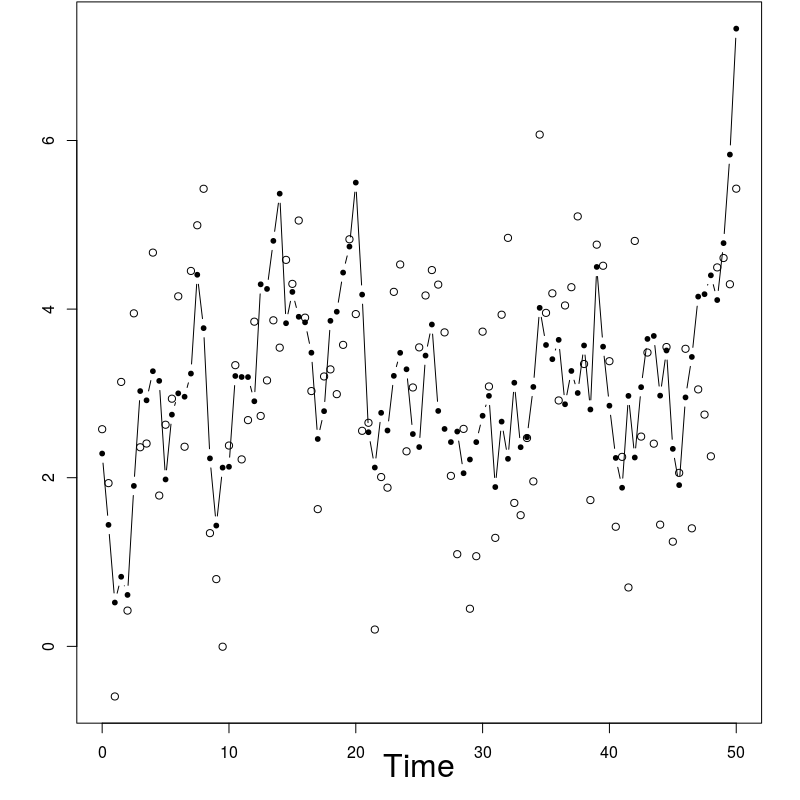
\includegraphics[width=0.8\textwidth]{obs_SINE.png}
\caption{Process $X$ solution to the SDE \eqref{eq:Lamp:SINE} (white) and observations $Y$ satisfying equation \eqref{eq:obs:SINE} (black) at times $t_0=0,\dots,t_{200}=200$.}
\label{fig:obs:SINE}
\end{figure}
\begin{figure}[p]
\centering
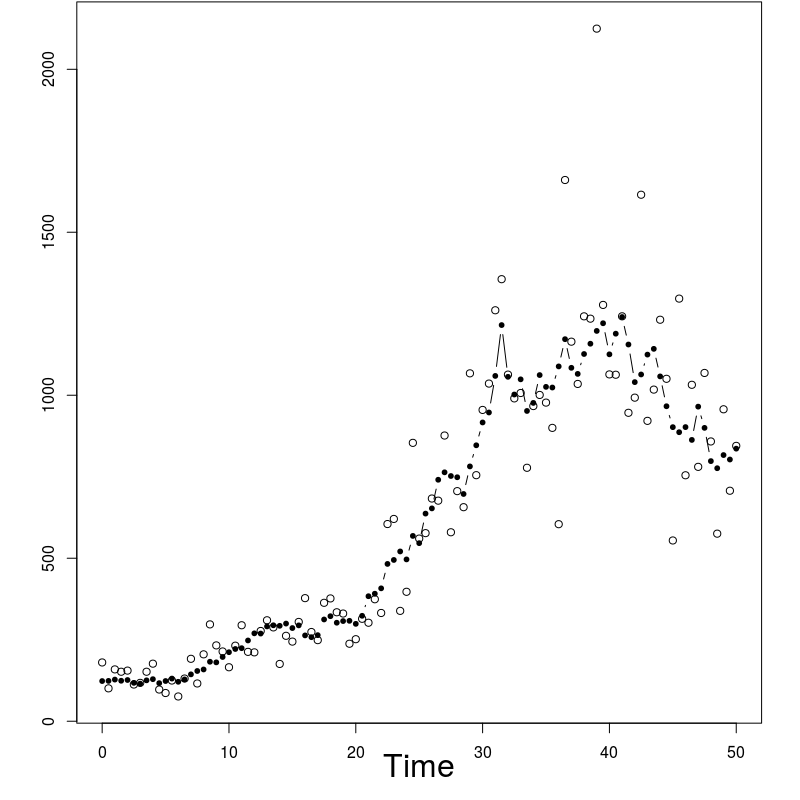
\includegraphics[width=0.8\textwidth]{obs_LG}
\caption{Process $X$ solution to the SDE \eqref{eq:Lamp:LG} (white) and observations $Y$ satisfying equation \eqref{eq:obs:LG}  (black) at times $t_0=0,\dots,t_{200}=100$.}
\label{fig:obs:LG}
\end{figure}
\begin{figure}[p]
\centering
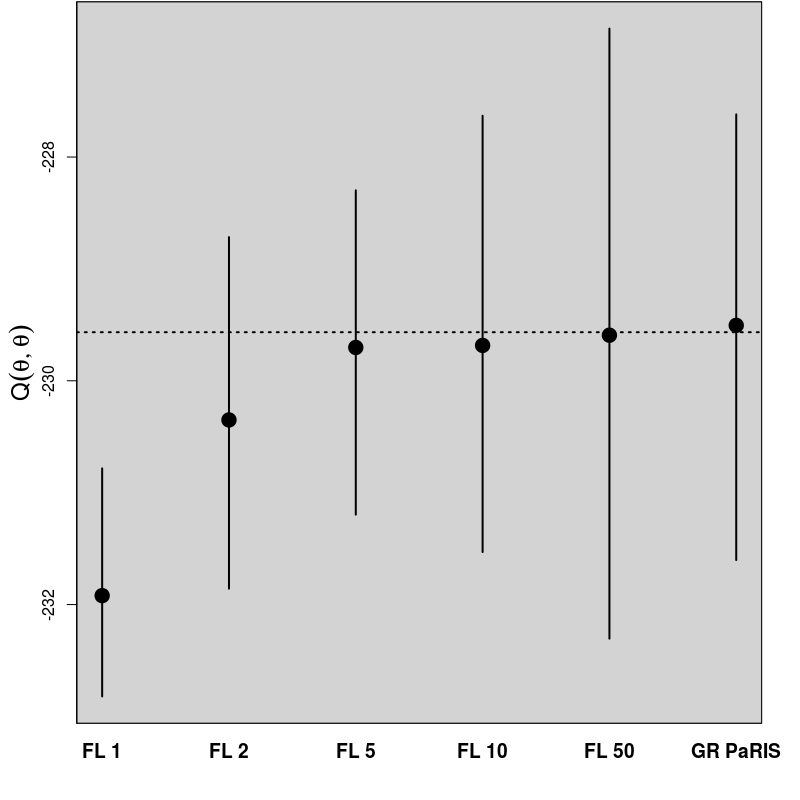
\includegraphics[width=0.8\textwidth]{res_Estep_SINE}
\caption{Estimation of the EM intermediate quantity $\mathcal{Q}(\theta_{true},\theta_{true})$ using observations of Figure \ref{fig:obs:SINE}, using the fixed lag (FL) technique for 5 different lags (namely 1, 2, 5,10 ,50), and the GRand PaRIS algorithm for the diffusion process proposed in this work, using 300 replicates. The whiskers represent the extent of the 95\% central values. The dot represents the empirical mean over the 300 replicates. The dotted line shows the reference value, computed using the unbiased GRand PaRIS algorithm with $N=10000$ particles.}
\label{fig:res:SINE}
\end{figure}
\begin{figure}[p]
\centering
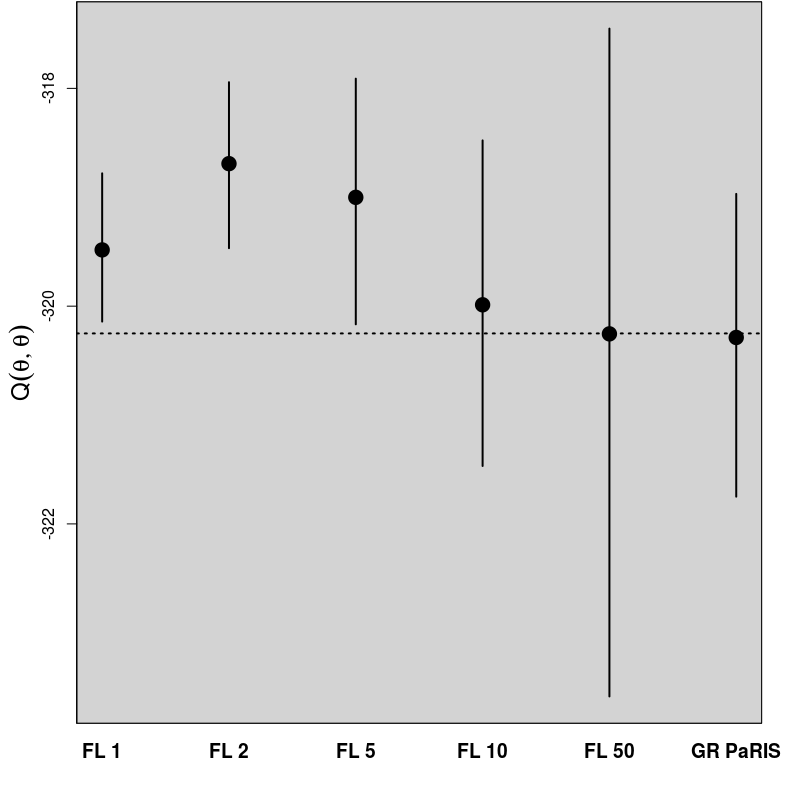
\includegraphics[width=0.8\textwidth]{res_Estep_LG}
\caption{Estimation of the EM intermediate quantity $\mathcal{Q}(\theta_{true},\theta_{true})$ using observations of Figure \ref{fig:obs:LG}, using the fixed lag (FL) technique for 5 different lags (namely 1, 2, 5,10 ,50), and the GRand PaRIS algorithm for the diffusion process proposed in this work, using 300 replicates. The whiskers represent the extent of the 95\% central values. The dot represents the empirical mean over the 300 replicates. The dotted line shows the reference value, computed using the unbiased GRand PaRIS algorithm with $N=10000$ particles.}
\label{fig:res:LG}
\end{figure}
\section{Conclusions}
This paper presents a new online SMC smoother for partially observed differential equations. This algorithm relies on an acceptance reject procedure inspired from the recent PaRIS algorithm. The main result of the article for practical applications is that the mechanism of this procedure remains valid when the transition density is approximated by a an unbiased positive estimator. The proposed procedure outperforms the existing fixed lag smoother for SDE of \cite{olsson:strojby:2011}, as it does not introduce intrinsic non vanishing bias,  and numerical simulations highlight a better variance on two examples. It can be implemented for the class of models $\mathcal{D}_1$ and $\mathcal{D}_2$ defined in \cite{beskos:papaspiliopoulos:roberts:fearnhead:2006} with a linear complexity in $N$. 
% where $\beta\in\mathbb{R}^d$ is chosen by the user. Assume that $\alpha_{\theta}$ is of the form $\alpha_{\theta}(x) = \nabla_x A_{\theta}(x)$ where $A_{\theta}: \mathbb{R}^d \to \mathbb{R}$. Writing $\mathbb{Q}_{\theta}$ (resp. $\mathbb{W}^{\beta}_{\theta}$) the probability measure induced by $(X_s)_{0\le s\le t}$  (resp. $(Y_s)_{0\le s\le t}$) on $(\mathsf{C},\mathcal{C})$, Girsanov theorem yields:
% \[
% \frac{\rmd \mathbb{Q}_{\theta}}{\rmd \mathbb{W}^{\beta}_{\theta}}(w) = \mathrm{exp}\left\{H_{\theta}(\omega_t) - H_{\theta}(\omega_0) - \frac{1}{2}\int_{0}^{t}\left\{\|\alpha_{\theta}(\mw_s)-\beta\|^2+\Delta H_{\theta}(\mw_s)\right\}\rmd s\right\}\eqsp,
% \]
% where $H_{\theta}(x) = A_{\theta}(x) -\beta'x$. Then, the probability measures conditioned on hitting $y$ at time $t$ satisfy:
% \[
% \frac{\rmd \mathbb{Q}^{y}_{\theta}}{\rmd \mathbb{W}^{\beta,y}_{\theta}}(w) = \frac{\varphi_t(y-x-t\beta)}{q^{t}_{\theta}(x,y)} \mathrm{exp}\left\{H_{\theta}(y) - H_{\theta}(x) - \frac{1}{2}\int_{0}^{t}\left\{\|\alpha_{\theta}(\mw_s)-\beta\|^2+\Delta H_{\theta}(\mw_s)\right\}\rmd s\right\}\eqsp.
% \]
% Assume also that for all $\theta$, there exists $\ell(\theta)$ such that:
% \[
% \mathrm{inf}_{u\in \mathbb{R}^d} \left\{\frac{1}{2}\left(\|\alpha_{\theta}(u)-\beta\|^2+\Delta H_{\theta}(u)\right)\right\}\ge \ell(\theta)\eqsp.
% \]
% Then
% \[
% q^{t}_{\theta}(x,y) = \varphi_t(y-x-t\beta)\eqsp\mathrm{exp}\left\{H_{\theta}(y) - H_{\theta}(x)+\ell(\theta)t\right\}\mathbb{E}_{\mathbb{W}^{\beta,y}}\left[\mathrm{exp}\left\{-\int_{0}^{t}\phi_{\theta}(\mw_s)\rmd s\right\}\right]\eqsp,
% \]
% where 
% \[
% \phi_{\theta}(x) = \frac{1}{2}\left\{\|\alpha_{\theta}(x)-\beta\|^2+\Delta H_{\theta}(x)\right\}-\ell(\theta)\eqsp.
% \]
% An unbiased estimator of $q^{t}_{\theta}(x,y)$ is then obtained by estimating $\mathbb{E}_{\mathbb{W}^{\beta,y}}\left[\mathrm{exp}\left\{-\int_{0}^{t}\phi_{\theta}(\mw_s)\rmd s\right\}\right]$.


% Let $h$ be a function defined on $\{1,\ldots,N\}$,
% \begin{align*}
% \mathbb{E}\left[h(I_{\tau})\right] & = \sum_{m\ge 0}\mathbb{E}\left[h(I_m)\1_{\tau=m}\right]\eqsp,\\
% & = \sum_{m\ge 0}h(m)\left(\prod_{\ell=0}^{m-1}\mathbb{E}\left[\1_{(\mathcal{A}^k_{\ell})^c}\right]\right)\mathbb{E}\left[h(I_m)\1_{\mathcal{A}^k_{m}}\right]\eqsp,\\
% & = \sum_{m\ge}\left(\prod_{\ell=0}^{m-1}\mathbb{E}\left[1-\frac{q^{\Delta t_k}_{\mathrm{GPE-1},\theta}(\kappa_{\ell},\omega^{\kappa_{\ell}},(U^{\kappa_{\ell}}_j)_{1\le j\le \kappa_{\ell}},\xi_{k-1}^{I_\ell},\xi_k^{1})}{M_{\theta}}\right]\right)\\
% &\hspace{5cm}\times\mathbb{E}\left[h(I_m)\frac{q^{\Delta t_k}_{\mathrm{GPE-1},\theta}(\kappa_{m},\omega^{\kappa_{m}},(U^{\kappa_{m}}_j)_{1\le j\le \kappa_{m}},\xi_{k-1}^{I_m},\xi_k^{1})}{M_{\theta}}\right]\eqsp,\\
% & = \sum_{m\ge 0}\left(\mathbb{E}\left[1-\frac{q^{\Delta t_k}_{\theta}(\xi_{k-1}^{I_1},\xi_k^{1})}{M_{\theta}}\right]\right)^m\mathbb{E}\left[h(I_m)\frac{q^{\Delta t_k}_{\theta}(\xi_{k-1}^{I_m},\xi_k^{1})}{M_{\theta}}\right]\eqsp,\\
% & = \mathbb{E}\left[h(I_1)q^{\Delta t_k}_{\theta}(\xi_{k-1}^{I_1},\xi_k^{1})\right]/\mathbb{E}\left[q^{\Delta t_k}_{\theta}(\xi_{k-1}^{I_m},\xi_k^{1})\right]\eqsp,\\
% & = \sum_{\ell=1}^N \frac{h(\ell)\omega_{k-1}^{\ell}q^{\Delta t_k}_{\theta}(\xi_{k-1}^{\ell},\xi_k^{1})}{\sum_{m=1}^N\omega_{k-1}^{m}q^{\Delta t_k}_{\theta}(\xi_{k-1}^{m},\xi_k^{1})}\eqsp,
% \end{align*}
% which concludes the proof.


\appendix

\section{Proofs}
\label{sec:append:proofs}
\begin{proof}[Proof of Lemma~\ref{lem:AR:unbiased}]
Let $\tau$ be the first time  draws are accepted in the accept-reject mechanism. For all $\ell\ge 1$, write
\[
\mathcal{A}^k_{\ell} = \left\{U_\ell<\widehat{q}_{k}(\xi_{k-1}^{J_\ell},\xi_k^{i},\zeta^{\ell}_{k})/\sigma_+\right\}\eqsp.
\]
Let $h$ be a function defined on $\{1,\ldots,N\}$,
\begin{align*}
\mathbb{E}\left[h(J^{i,j}_k)\middle| \mathcal{F}_k^N\right] & = \sum_{m\ge 1}\mathbb{E}\left[h(J_m)\1_{\tau=m}\middle| \mathcal{F}_k^N\right]\eqsp,\\
& = \sum_{m\ge 1}h(m)\left(\prod_{\ell=1}^{m-1}\mathbb{E}\left[\1_{(\mathcal{A}^k_{\ell})^c}\middle| \mathcal{F}_k^N\right]\right)\mathbb{E}\left[h(J_m)\1_{\mathcal{A}^k_{m}}\middle| \mathcal{F}_k^N\right]\eqsp,\\
& = \sum_{m\ge 1}\left(\prod_{\ell=1}^{m-1}\mathbb{E}\left[1-\frac{\widehat{q_k}(\xi_{k-1}^{J_\ell},\xi_k^{i};\zeta_k^{\ell})}{\hat{\sigma}_{+}}\middle| \mathcal{F}_k^N\right]\right)\\
&\hspace{5cm}\times\mathbb{E}\left[h(I_m)\frac{\widehat{q_k}(\xi_{k-1}^{J_m},\xi_k^{i};\zeta_k^{\ell})}{\hat{\sigma}_{+}}\middle| \mathcal{F}_k^N\right]\eqsp,\\
& = \sum_{m\ge 1}\left(\mathbb{E}\left[1-\frac{q_k(\xi_{k-1}^{J_1},\xi_k^{1})}{\hat{\sigma}_{+}}\middle| \mathcal{F}_k^N\right]\right)^{m-1}\mathbb{E}\left[h(J_m)\frac{q_k(\xi_{k-1}^{J_m},\xi_k^{1})}{\hat{\sigma}_{+}}\middle| \mathcal{F}_k^N\right]\eqsp,\\
& = \mathbb{E}\left[h(J_1)q_k(\xi_{k-1}^{J_1},\xi_k^{i})\middle| \mathcal{F}_k^N\right]/\mathbb{E}\left[q_k(\xi_{k-1}^{J_m},\xi_k^{i})\middle| \mathcal{F}_k^N\right]\eqsp,\\
& = \sum_{\ell=1}^N \frac{h(\ell)\omega_{k-1}^{\ell}q_k(\xi_{k-1}^{\ell},\xi_k^{i})}{\sum_{m=1}^N\omega_{k-1}^{m}q_k(\xi_{k-1}^{m},\xi_k^{i})}\eqsp,\\
&= \sum_{\ell=1}^N \Lambda_{k-1}^N(i,\ell)h(\ell) \eqsp,
\end{align*}
which concludes the proof.

%The goal is to simulate realisations of  a discrete random variable $X$ having the following target distribution:
%\begin{equation}
%\mP(X=\ell)= p_X(\ell)=\frac{\omega_k^\ell q_k(\xi_k^\ell,\xi_{k+1})}{\sum_{\ell=1}^N\omega_k^\ell q_k(\xi_k^\ell,\xi_{k+1})},~~\ell\in \{1,\dots,N\}
%\end{equation}
%for some $\xi_{k+1}$ that has no importance in this result. We assume $\omega_k$ are normalized weights, i.e. $\sum_\ell \omega_k^l=1$. The candidate will therefore be sampled from $Y$, a r.v. with the following distribution:
%\begin{equation}
%\mP(Y=\ell)=p_Y(\ell)= \omega_k^\ell,~~\ell\in \{1,\dots,N\}
%\end{equation}
%Unfortunately, the $q_k$ function is unknown. Howevere, we let's suppose we can define an unbiased estimator $\hat{q}_k(\xi_k^\ell,\xi_{k+1},\zeta)$, where $\zeta$ is a random variable having th p.d.f. $p_\zeta$.  We have therefore:
%$$\E_{p_\zeta}\left[\hat{q}_k(\xi_k^\ell,\xi_{k+1},\zeta)\right]=q(\xi_k^\ell,\xi_{k+1})$$
%Moreover, we impose the following property over this estimator, we want that:
%$$\exists \sigma_+\in \mathbb{R}\text{ such that }\forall x,y,~~\hat{q}_k(x,y,\zeta)\leq \sigma_+$$
%To simulate a random variable $X\sim p_X$, we propose the following algorithm:
%\begin{enumerate}
%\item Sample independently $\ell\sim p_Y$, $z\sim p_\zeta$ and $u \sim \mathcal{U}[0,1]$
%\item \textbf{If} 
%$$u \leq \frac{\hat{q}_k(\xi_k^\ell,\xi_{k+1},z)}{\sigma_+},$$
%set $x=\ell$. \textbf{Else}, return to 1).
%\end{enumerate}



%The lemma \ref{lem:AR:unbiased} states that $x$ is a realisation of a random variable $X\sim p_X$. Indeed
%\begin{align*}
%\mP\left(Y=\ell\vert U\leq \frac{\hat{q}_k(\xi_k^Y,\xi_{k+1},\zeta)}{\sigma_+}\right)&=\frac{\mP\left(U\leq \frac{\hat{q}_k(\xi_k^Y,\xi_{k+1},\zeta)}{\sigma_+}\vert Y=l \right) \mathbb{P}(Y=\ell)}{\mP\left(U\leq \frac{\hat{q}_k(\xi_k^Y,\xi_{k+1},\zeta)}{\sigma_+}\right)}\\
%&=\frac{\mP\left(U\leq \frac{\hat{q}_k(\xi_k^\ell,\xi_{k+1},\zeta)}{\sigma_+} \right) \omega_k^\ell}{\mP\left(U\leq \frac{\hat{q}_k(\xi_k^Y,\xi_{k+1},\zeta)}{\sigma_+}\right)}
%\intertext{We now note that}
%\mP\left(U\leq \frac{\hat{q}_k(\xi_k^Y,\xi_{k+1},\zeta)}{\sigma_+}\right)&=\E_{p_\zeta}\left[\E\left[\E_{p_Y}\left[\E\left[\mP\left(U\leq \frac{\hat{q}_k(\xi_k^Y,\xi_{k+1},\zeta)}{\sigma_+}\right) \vert Y\right] \right] \vert \zeta\right]\right]\\
%&=\E_{p_\zeta}\left[\sum_{\ell=1}^N w_k^l\frac{\hat{q}_k(\xi_k^\ell,\xi_{k+1},\zeta)}{\sigma_+} \right]~~(\text{As }\frac{\hat{q}_k(\xi_k^Y,\xi_{k+1},\zeta)}{\sigma_+}\leq 1)\\
%&=\frac{1}{\sigma_+}\sum_{\ell=1}^N w_k^\ell q_k(\xi_k^\ell,\xi_{k+1})
%\intertext{In the same way, we have:}
%\mP\left(U\leq \frac{\hat{q}_k(\xi_k^\ell,\xi_{k+1},\zeta)}{\sigma_+}\right)&=\frac{1}{\sigma_+} q_k(\xi_k^\ell,\xi_{k+1})
%\intertext{Which gives overall the wanted result}
%\mP\left(Y=\ell\vert U\leq \frac{\hat{q}_k(\xi_k^Y,\xi_{k+1},\zeta)}{\sigma_+}\right)&=\frac{\omega_k^\ell q_k(\xi_k^\ell,\xi_{k+1})}{\sum_{l=1}^N w_k^\ell q_k(\xi_k^\ell,\xi_{k+1})}=p_X(\ell),~~\ell\in \{1,\dots,N\}
%\end{align*}
%\end{proof}
\end{proof}


\begin{proof}[Proof of Lemma \ref{lem:iid}]
The independence is ensured by the mechanism of SMC methods. By \eqref{eq:random:weight},
\[
\mathbb{E}\left[\widehat{\omega}^i_{k+1}\tau^{i}_{k+1}\middle| \mathcal{F}_k^{N}\right] = \mathbb{E}\left[\frac{ \widehat{\qk}(\xi_{k}^{I^{i}_{k+1}}, \xi^{i}_{k+1};\zeta_{k+1})g_{k+1}(\xi^{i}_{k+1})}{\vartheta_{k+1}(\xi^{I^{i}_{k+1}}_{k}) p_{k+1}(\xi_{k}^{I^{i}_{k+1}},\xi^{i}_{k+1})}\tau^{i}_{k+1}\middle| \mathcal{F}_k^{N}\right]\eqsp.
%&= \mathbb{E}\left[\frac{g_{k+1}(\xi^{1}_{k+1})}{\vartheta_{k+1}(\xi^{I^{1}_{k+1}}_{k}) p_{k+1}(\xi_{k}^{I^{1}_{k+1}},\xi^{\ell}_{k+1})}\tau^{1}_{k+1}\widehat{q}_{\theta}^{\Delta t_{k+1}}(\xi_{k}^{I^{1}_{k+1}},\xi^{1}_{k+1};\Lambda_{k+1})\middle| \mathcal{F}_k^{N}\right]\eqsp,
\]
Note that
\begin{align*}
&\mathbb{E}\left[\tau^{i}_{k+1}\middle|\sigma\left(\mathcal{F}_k^{N},\{\xi_{k+1}^i,I_{k+1}^i\}\right)\right]
 = \sum_{\ell=1}^N\frac{\omega_k^{\ell} \qk(\xi_{k}^{\ell}, \xi^{i}_{k+1}) \left(\tau^{\ell}_k + h_{k}(\xi_{k}^{\ell},\xi^{i}_{k+1})\right)}{\sum_{\ell'=1}^N\omega_k^{\ell'} \qk(\xi_{k}^{\ell'},\xi^{i}_{k+1})}\eqsp,\\
&\mathbb{E} \left[\widehat{\qk}(\xi_{k}^{I^{i}_{k+1}},\xi^{i}_{k+1};\zeta_{k+1}) \middle| \sigma \left(\mathcal{F}_k^{N},\{\xi_{k+1}^i,I^{i}_{k+1}\}\right)\right]
 = \qk(\xi_{k}^{I^{i}_{k+1}},\xi^{i}_{k+1})\eqsp.
\end{align*}
Since $\tau^{i}_{k+1}$ and $\zeta_{k+1}$ are independent conditionally to $\sigma\left(\mathcal{F}_k^{N},\{\xi_{k+1}^{\ell}, I_{k+1}^{\ell}\}_{\ell=1}^N\right)$:
\begin{multline*}
\mathbb{E}\left[\tau^{i}_{k+1} \widehat{\qk} (\xi_{k}^{I^{i}_{k+1}},\xi^{i}_{k+1};\zeta_{k+1})\middle|\sigma\left(\mathcal{F}_k^{N},\{\xi_{k+1}^i,I_{k+1}^i\} \right)\right]\\
 = q_k(\xi_{k}^{I^{i}_{k+1}},\xi^{i}_{k+1})\sum_{\ell=1}^N\frac{\omega_k^{\ell} \qk (\xi_{k}^{\ell},\xi^{i}_{k+1})\left(\tau^{\ell}_k + h_{k}(\xi_{k}^{\ell},\xi^{i}_{k+1})\right)}{\sum_{\ell'=1}^N\omega_k^{\ell'} \qk (\xi_{k}^{\ell'},\xi^{i}_{k+1})}\eqsp.
\end{multline*}
Moreover, conditionally to $\mathcal{F}_k^N$, the probability density function of $(\xi_{k+1}^i,I_{k+1}^i)$ is given by
\[
(x,j) \mapsto \frac{\omega_k^j\vartheta_{k+1}(\xi_k^j)p_k(\xi_k^j,x)}{\Omega_k\phi_k^N[\vartheta_{k+1}]}\eqsp.
\]
Therefore, this yields:
\begin{align*}
\mathbb{E}\left[\widehat{\omega}^i_{k+1}\tau^{i}_{k+1}\middle| \mathcal{F}_k^{N}\right]&= \left(\phi^N_{k}[\vartheta_{k+1}]\right)^{-1} \sum_{j=1}^N\frac{\omega_k^j}{\Omega_k} \int \vartheta_{k+1}(\xi^{j}_{k})\frac{\qk(\xi_{k}^{j},x) g_{k+1}(x)}{\vartheta_{k+1}(\xi^{j}_{k}) p_{k}(\xi_{k}^{j},x)}\\
&\hspace{1cm}\times \sum_{\ell=1}^N\frac{\omega_k^{\ell} \qk (\xi_{k}^{\ell},x)\left(\tau^{\ell}_k + h_{k}(\xi_{k}^{\ell},x)\right)}{\sum_{\ell'=1}^N\omega_k^{\ell'}\qk(\xi_{k}^{\ell'},x)}p_{k}(\xi_{k}^{j},x)\rmd x\eqsp,\\
&= \left(\phi^N_{k}[\vartheta_{k+1}]\right)^{-1}\\
&~~~~\times\sum_{\ell=1}^N \frac{\omega_k^\ell}{\Omega_k}\left[\int \frac{ \sum_{j=1}^N \omega_k^j\qk(\xi_k^j,x) }{ \sum_{\ell'=1}^N\omega_k^{\ell'}\qk(\xi_{k}^{\ell'},x) } g_{k+1}(x)\qk (\xi_{k}^{\ell},x)\left(\tau^{\ell}_k + h_{k}(\xi_{k}^{\ell},x)\right) \rmd x \right]\\ 
& =\left(\phi^N_{k}[\vartheta_{k+1}]\right)^{-1}\phi^N_{k}\left[\int \qk(\cdot,x)g_{k+1}(x)\left\{\tau_k(\cdot) + h_{k}(\cdot,x)\right\}\rmd x\right]\eqsp,
\end{align*}
which concludes the proof.
\end{proof}

%\section{Multidimensional Ornstein Uhlenbeck bridge}
%\label{sec:ornstein:bridge}
%The GPE introduced in this paper requires to sample finite dimensional distributions of Ornstein Uhlenbeck bridges. These results are given here for completeness. Consider the following $d$-dimensional SDE:
%\begin{equation}
%\label{eq:sde:ornstein}
%Z_0 = z_0\quad\mbox{and}\quad \rmd Z_t = (\Upsilon Z_t + \vartheta)\rmd t + \rmd W_t\eqsp,
%\end{equation}
%where $W$ is a standard Brownian motion on $\mathbb{R}^d$, $A$ is a $d\times d$ matrix and $b$ a $d$ dimensional vector. In the case of Section~\ref{sec:PaRIS:SDE}, for all $1\le k \le n$, the proposal stochastic differential equation governing $Y_t^k$, $t\in(t_{k-1},t_k)$, is of the form \eqref{eq:sde:ornstein} with
%\[
%\Upsilon = J_{\alpha_{\theta}}(X_{k-1})\;\;\mbox{and}\;\; \vartheta =\alpha_{\theta}(X_{k-1}) - J_{\alpha_{\theta}}(X_{k-1})X_{k-1}\eqsp,
%\]
%$J_{\alpha_{\theta}}$ being the Jacobian of $\alpha_{\theta}$. In this case, as $\alpha_{\theta}(x) = \nabla_x A_{\theta}(x)$, $A$ is symmetric and nonsingular. By \cite[Section~5.6]{karatzas:shreve:1991}, the unique strong solution of \eqref{eq:sde:ornstein} is:
%\[
%Z_t = \mathrm{e}^{t\Upsilon}z_0 + \int_0^t\mathrm{e}^{(t-s)\Upsilon}\vartheta \rmd s + \int_0^t\mathrm{e}^{(t-s)\Upsilon} \rmd W_s\eqsp.
%\]
%Therefore, the probability density of the conditional distribution of $Z_t$ given $Z_0 = z_0$ is Gaussian with mean $\mu_t(z_0)$ and variance $\Sigma_{t}$ given by:
%\begin{align*}
%\Sigma_{t} &= \int_0^{t} \mathrm{e}^{(t -s)\Upsilon}\mathrm{e}^{(t -s)\Upsilon'}\rmd s\eqsp,\\
%\mu_{t}(z) &= \mathrm{e}^{t \Upsilon}z_0 + \left(\int_0^t\mathrm{e}^{(t-s)\Upsilon} \rmd s\right)\vartheta\eqsp.
%\end{align*}
%As $\Upsilon$ is symetric and nonsingular,
%\begin{align*}
%\Sigma_{t} &= \int_0^{t} \mathrm{e}^{2(t -s)\Upsilon}\rmd s = \Upsilon^{-1}(\mathrm{e}^{2t\Upsilon}-I_d)/2\eqsp,\\
%\mu_{t}(z) &= \mathrm{e}^{t \Upsilon}z + \left(\int_0^t\mathrm{e}^{(t-s)\Upsilon} \rmd s\right)\vartheta = \mathrm{e}^{t \Upsilon}z + \Upsilon^{-1}(\mathrm{e}^{t\Upsilon}-I_d)\vartheta \eqsp.
%\end{align*}
%For each interval $(t_{k-1},t_k)$, $1\le k \le n$, the GPE requires to sample a Ornstein-Uhlenbeck bridge at some ramdom time steps between $X_{k-1}$ at time $t_{k-1}$ and $X_k$ at time $t_k$. Conditional on $Z_s = x$ and $Z_T = y$, the probability density of $Z_t$ is Gaussian with mean $\mu$ and variance $\Sigma_t^{s,T}$ given by: 
%\begin{align*}
%\mu &=\Gamma(t,T)\Gamma(s,T)^{-1}\mu_- + \Gamma(s,t)'(\Gamma(s,T)')^{-1}\mu_+\eqsp,\\
%\Sigma_t^{s,T} &=\Gamma(t,T)\Gamma(s,T)^{-1}\Gamma(s,t)\eqsp,\\
%\Gamma(s,t)&=\int_s^{t} \mathrm{e}^{(s -u)\Upsilon}\mathrm{e}^{(t -u)\Upsilon'}\rmd u\eqsp = \Upsilon^{-1}\left(\mathrm{e}^{(t -s)\Upsilon}-\mathrm{e}^{(s -t)\Upsilon}\right)/2\eqsp,\\
%\mu_- &= x - \Upsilon^{-1}(\mathrm{e}^{(s -t)\Upsilon}-I_d)\vartheta\eqsp,\\
%\mu_+ &= y-\Upsilon^{-1}(\mathrm{e}^{(T -t)\Upsilon}-I_d)\vartheta\eqsp.
%\end{align*}

\begin{proof}[Proof of Proposition~\ref{prop:exp:deviation}]
The results is proved by induction. At time $k=0$, the result holds using that for all $1\le i \le N$, $\rho_0^i = 0$ and the convention $T_0[h_0] =0$. In addition, $\phi_0^N$ is a standard importance sampler estimator of $\phi_0$ with $\omega_0^i\le |\widehat{\omega}_0|_{\infty}$ so that for any bounded function $h$ on $\mathsf{X}$,
\[
\mathbb{P}\left(\left|\phi_0^N[h] - \phi_0\left[h\right]\right|\ge \varepsilon\right)\le b_0\exp\left(-c_0N\varepsilon^2\right)\eqsp.
\]
Assume the results holds for $k\ge 1$ and that $\vartheta_{k+1} = 1$ for simplicity. Write
\[
\phi_{k+1}^N[\tau_{k+1}] - \phi_{k+1}\left[T_{k+1}[h_{k+1}]\right] = a_N/b_N\eqsp,
\]
where $a_N = N^{-1}\sum_{i=1}^N \widehat{\omega}_{k+1}^i \left(\tau_{k+1}^i - \phi_{k+1}\left[T_{k+1}[h_{k+1}]\right]\right)$ and $b_N =N^{-1}\sum_{i=1}^N \widehat{\omega}_{k+1}^i$. By Lemma~\ref{lem:iid}, the random variables $\{\widehat{\omega}_{k+1}^i\tau_{k+1}^i\}_{i=1}^N$ are independent conditionally on $\mathcal{F}_k^{N}$ and by H\ref{assum:boundalgo},
\[
\left|\widehat{\omega}_{k+1}^i \left(\tau_{k+1}^i - \phi_{k+1}\left[T_{k+1}[h_{k+1}]\right]\right)\right| \le 2|\widehat{\omega}_{k+1}|_{\infty}|H_{k+1}|_{\infty}\eqsp.
\]
Therefore, by Hoeffding inequality,
\[
\mathbb{P}\left(\left|a_N - \mathbb{E}\left[a_N\middle|\mathcal{F}_k^{N}\right]\right|\ge \varepsilon\right) = \mathbb{E}\left[\mathbb{P}\left(\left|a_N - \mathbb{E}\left[a_N\middle|\mathcal{F}_k^{N}\right]\right|\ge \varepsilon\middle|\mathcal{F}_k^{N}\right)\right]\le 2\exp\left(-c_kN\varepsilon^2\right)\eqsp.
\] 
On the other hand,
\[
%\mathbb{E}\left[a_N\middle|\mathcal{F}_k^{N}\right] = \left(\phi^N_{k}[\vartheta_{k+1}]\right)^{-1}\phi^N_{k}\left[\Upsilon_k\right] \eqsp,
\mathbb{E}\left[a_N\middle|\mathcal{F}_k^{N}\right] = \phi^N_{k}\left[\Upsilon_k\right] \eqsp,
\]
where
\[
\Upsilon_k(x_k) = \int q_{k}(\cdot,x)g_{k+1}(x)\left(\tau_k(x_k) + h_{k+1}(x_k,x) - \phi_{k+1}\left[T_{k+1}[h_{k+1}]\right]\right)\rmd x\eqsp.
\]
By \cite[Lemma~11]{olsson:westerborn:2016}, $\phi_{k}\left[\Upsilon_k\right] = 0$ which implies by the induction assumption that 
\[
\mathbb{P}\left(\left|\mathbb{E}\left[a_N\middle|\mathcal{F}_k^{N}\right]\right|\ge \varepsilon\right)\le b_k\exp\left(-c_kN\varepsilon^2\right)\eqsp.
\]
Then,
\[
\mathbb{P}\left(\left|a_N\right|\ge \varepsilon\right) \le b_k\exp\left(-c_kN\varepsilon^2\right)\eqsp.
\] 
Similarly, as $b_N \le |\widehat{\omega}_k|_{\infty}$, by Hoeffding inequality,
\begin{multline*}
\mathbb{P}\left(\left|b_N - \mathbb{E}\left[b_N\middle|\mathcal{F}_k^{N}\right]\right|\ge \varepsilon\right) \\
= \mathbb{E}\left[\mathbb{P}\left(\left|b_N - \mathbb{E}\left[b_N\middle|\mathcal{F}_k^{N}\right]\right|\ge \varepsilon\middle|\mathcal{F}_k^{N}\right)\right]\le 2\exp\left(-c_kN\varepsilon^2\right)\eqsp.
\end{multline*}
Note that
\[
\mathbb{E}\left[b_N\middle|\mathcal{F}_k^{N}\right] = \phi^N_{k}\left[\int q_{k}(\cdot,x)g_{k+1}(x)\rmd x\right]\eqsp.
\]
By  the induction assumption,
\[
\mathbb{P}\left(\left|\mathbb{E}\left[b_N\middle|\mathcal{F}_k^{N}\right]-\phi_k\left[\int q_{k}(\cdot,x)g_{k+1}(x)\rmd x\right]\right|\ge \varepsilon\right)\le b_k\exp\left(-c_kN\varepsilon^2\right)\eqsp.
\]
The proof is completed using Lemma~\ref{lem:hoeffding:ratio}.
\end{proof}


\begin{lemma}\label{lem:hoeffding:ratio}
Assume that $a_N$, $b_N$, and $b$ are random variables defined on the same probability space such that there exist positive constants $\beta$, $B$, $C$, and $M$ satisfying
\begin{enumerate}[(i)]
    \item $|a_N/b_N|\leq M$, $\mathbb{P}$-a.s.\ and  $b \geq \beta$, $\mathbb{P}$-a.s.,
    \item For all $\epsilon>0$ and all $N\geq1$, $\mathbb{P}\left[|b_N-b|>\epsilon \right]\leq B \exp\left(-C N \epsilon^2\right)$,
    \item For all $\epsilon>0$ and all $N\geq1$, $\mathbb{P} \left[ |a_N|>\epsilon \right]\leq B \exp\left(-C N \left(\epsilon/M\right)^2\right)$.
\end{enumerate}
Then,
$$
    \mathbb{P}\left\{ \left| \frac{a_N}{b_N} \right| > \epsilon \right\} \leq B \exp{\left(-C N \left(\frac{\epsilon \beta}{2M} \right)^2 \right)} \eqsp.
$$
\end{lemma}
\begin{proof}
See \cite{douc:garivier:moulines:olsson:2011}.
\end{proof}



\bibliographystyle{plain}
\bibliography{./ParisEM_bib}
\end{document}